% Options for packages loaded elsewhere
\PassOptionsToPackage{unicode}{hyperref}
\PassOptionsToPackage{hyphens}{url}
\PassOptionsToPackage{dvipsnames,svgnames,x11names}{xcolor}
%
\documentclass[
  article]{jss}

\usepackage{amsmath,amssymb}
\usepackage{iftex}
\ifPDFTeX
  \usepackage[T1]{fontenc}
  \usepackage[utf8]{inputenc}
  \usepackage{textcomp} % provide euro and other symbols
\else % if luatex or xetex
  \usepackage{unicode-math}
  \defaultfontfeatures{Scale=MatchLowercase}
  \defaultfontfeatures[\rmfamily]{Ligatures=TeX,Scale=1}
\fi
\usepackage{lmodern}
\ifPDFTeX\else  
    % xetex/luatex font selection
\fi
% Use upquote if available, for straight quotes in verbatim environments
\IfFileExists{upquote.sty}{\usepackage{upquote}}{}
\IfFileExists{microtype.sty}{% use microtype if available
  \usepackage[]{microtype}
  \UseMicrotypeSet[protrusion]{basicmath} % disable protrusion for tt fonts
}{}
\makeatletter
\@ifundefined{KOMAClassName}{% if non-KOMA class
  \IfFileExists{parskip.sty}{%
    \usepackage{parskip}
  }{% else
    \setlength{\parindent}{0pt}
    \setlength{\parskip}{6pt plus 2pt minus 1pt}}
}{% if KOMA class
  \KOMAoptions{parskip=half}}
\makeatother
\usepackage{xcolor}
\setlength{\emergencystretch}{3em} % prevent overfull lines
\setcounter{secnumdepth}{-\maxdimen} % remove section numbering
% Make \paragraph and \subparagraph free-standing
\ifx\paragraph\undefined\else
  \let\oldparagraph\paragraph
  \renewcommand{\paragraph}[1]{\oldparagraph{#1}\mbox{}}
\fi
\ifx\subparagraph\undefined\else
  \let\oldsubparagraph\subparagraph
  \renewcommand{\subparagraph}[1]{\oldsubparagraph{#1}\mbox{}}
\fi


\providecommand{\tightlist}{%
  \setlength{\itemsep}{0pt}\setlength{\parskip}{0pt}}\usepackage{longtable,booktabs,array}
\usepackage{calc} % for calculating minipage widths
% Correct order of tables after \paragraph or \subparagraph
\usepackage{etoolbox}
\makeatletter
\patchcmd\longtable{\par}{\if@noskipsec\mbox{}\fi\par}{}{}
\makeatother
% Allow footnotes in longtable head/foot
\IfFileExists{footnotehyper.sty}{\usepackage{footnotehyper}}{\usepackage{footnote}}
\makesavenoteenv{longtable}
\usepackage{graphicx}
\makeatletter
\def\maxwidth{\ifdim\Gin@nat@width>\linewidth\linewidth\else\Gin@nat@width\fi}
\def\maxheight{\ifdim\Gin@nat@height>\textheight\textheight\else\Gin@nat@height\fi}
\makeatother
% Scale images if necessary, so that they will not overflow the page
% margins by default, and it is still possible to overwrite the defaults
% using explicit options in \includegraphics[width, height, ...]{}
\setkeys{Gin}{width=\maxwidth,height=\maxheight,keepaspectratio}
% Set default figure placement to htbp
\makeatletter
\def\fps@figure{htbp}
\makeatother

\usepackage{orcidlink,thumbpdf,lmodern}

\newcommand{\class}[1]{`\code{#1}'}
\newcommand{\fct}[1]{\code{#1()}}
\makeatletter
\@ifpackageloaded{tcolorbox}{}{\usepackage[skins,breakable]{tcolorbox}}
\@ifpackageloaded{fontawesome5}{}{\usepackage{fontawesome5}}
\definecolor{quarto-callout-color}{HTML}{909090}
\definecolor{quarto-callout-note-color}{HTML}{0758E5}
\definecolor{quarto-callout-important-color}{HTML}{CC1914}
\definecolor{quarto-callout-warning-color}{HTML}{EB9113}
\definecolor{quarto-callout-tip-color}{HTML}{00A047}
\definecolor{quarto-callout-caution-color}{HTML}{FC5300}
\definecolor{quarto-callout-color-frame}{HTML}{acacac}
\definecolor{quarto-callout-note-color-frame}{HTML}{4582ec}
\definecolor{quarto-callout-important-color-frame}{HTML}{d9534f}
\definecolor{quarto-callout-warning-color-frame}{HTML}{f0ad4e}
\definecolor{quarto-callout-tip-color-frame}{HTML}{02b875}
\definecolor{quarto-callout-caution-color-frame}{HTML}{fd7e14}
\makeatother
\makeatletter
\makeatother
\makeatletter
\makeatother
\makeatletter
\@ifpackageloaded{caption}{}{\usepackage{caption}}
\AtBeginDocument{%
\ifdefined\contentsname
  \renewcommand*\contentsname{Table of contents}
\else
  \newcommand\contentsname{Table of contents}
\fi
\ifdefined\listfigurename
  \renewcommand*\listfigurename{List of Figures}
\else
  \newcommand\listfigurename{List of Figures}
\fi
\ifdefined\listtablename
  \renewcommand*\listtablename{List of Tables}
\else
  \newcommand\listtablename{List of Tables}
\fi
\ifdefined\figurename
  \renewcommand*\figurename{Figure}
\else
  \newcommand\figurename{Figure}
\fi
\ifdefined\tablename
  \renewcommand*\tablename{Table}
\else
  \newcommand\tablename{Table}
\fi
}
\@ifpackageloaded{float}{}{\usepackage{float}}
\floatstyle{ruled}
\@ifundefined{c@chapter}{\newfloat{codelisting}{h}{lop}}{\newfloat{codelisting}{h}{lop}[chapter]}
\floatname{codelisting}{Listing}
\newcommand*\listoflistings{\listof{codelisting}{List of Listings}}
\makeatother
\makeatletter
\@ifpackageloaded{caption}{}{\usepackage{caption}}
\@ifpackageloaded{subcaption}{}{\usepackage{subcaption}}
\makeatother
\makeatletter
\makeatother
\ifLuaTeX
  \usepackage{selnolig}  % disable illegal ligatures
\fi
\IfFileExists{bookmark.sty}{\usepackage{bookmark}}{\usepackage{hyperref}}
\IfFileExists{xurl.sty}{\usepackage{xurl}}{} % add URL line breaks if available
\urlstyle{same} % disable monospaced font for URLs
\hypersetup{
  pdftitle={Imputation of Incomplete Multilevel Data with R},
  pdfauthor={Hanne I. Oberman; Johanna Muñoz; Valentijn M.T. de Jong; Gerko Vink; Thomas P.A. Debray},
  pdfkeywords={missing data, multilevel, clustering, mice, R},
  colorlinks=true,
  linkcolor={blue},
  filecolor={Maroon},
  citecolor={Blue},
  urlcolor={Blue},
  pdfcreator={LaTeX via pandoc}}

%% -- Article metainformation (author, title, ...) -----------------------------

%% Author information
\author{Hanne I. Oberman~\orcidlink{0000-0003-3276-2141}\\Utrecht
University \And Johanna
Muñoz~\orcidlink{0000-0002-2384-5415}\\University Medical Center
Utrecht \AND Valentijn M.T. de
Jong~\orcidlink{0000-0001-9921-3468}\\University Medical Center
Utrecht \And Gerko Vink~\orcidlink{0000-0001-9767-1924}\\University
Medical Center Utrecht \AND Thomas P.A.
Debray~\orcidlink{0000-0002-1790-2719}\\University Medical Center
Utrecht}
\Plainauthor{Hanne I. Oberman, Johanna Muñoz, Valentijn M.T. de
Jong, Gerko Vink, Thomas P.A. Debray} %% comma-separated

\title{Imputation of Incomplete Multilevel Data with R}
\Plaintitle{Imputation of Incomplete Multilevel Data with
R} %% without formatting

%% an abstract and keywords
\Abstract{This tutorial illustrates the imputation of incomplete
multilevel data with the \proglang{R} packackage \pkg{mice}. Our scope
is only simple multilevel models, to show how imputation can yield less
biased estimates from incomplete clustered data. More complex models can
be accomodated, but are outside the scope of this paper. Incomplete
multilevel data requires careful consideration of the missing data
problem and analysis strategy. In this tutorial, we focus on a popular
strategy for accommodating missingness in multilevel data: replacing the
missing data with one or more plausible values, i.e.,
imputation.Imputation separates the missing data problem from the main
analysis and the completed data can be analyzed as if it has been fully
observed. This tutorial illustrates the imputation of incomplete
multilevel data with the statistical programming language R. We aim to
show how imputation can yield less biased estimates from incomplete
clustered data. We provide practical guidelines and code snippets for
different missing data situations, including non-ignorable missingness
mechanisms. For brevity, we focus on multilevel imputation using chained
equations with the R mice package and its adjacent packages.}

%% at least one keyword must be supplied
\Keywords{missing
data, multilevel, clustering, \pkg{mice}, \proglang{R}}
\Plainkeywords{missing data, multilevel, clustering, mice, R}

%% publication information
%% NOTE: Typically, this can be left commented and will be filled out by the technical editor
%% \Volume{50}
%% \Issue{9}
%% \Month{June}
%% \Year{2012}
%% \Submitdate{2012-06-04}
%% \Acceptdate{2012-06-04}
%% \setcounter{page}{1}
%% \Pages{1--xx}

%% The address of (at least) one author should be given
%% in the following format:
\Address{
Hanne I. Oberman\\
Methodology and Statistics\\
Padualaan 14\\
Utrecht The Netherlands\\
E-mail: \email{h.i.oberman@uu.nl}\\
URL: \url{https://www.hanneoberman.github.io}\\
\\~
Johanna Muñoz\\
Julius Centre for Health Sciences and Primary Care\\
Universiteitsweg 100\\
Utrecht The Netherlands\\
\\~
Valentijn M.T. de Jong\\
Julius Centre for Health Sciences and Primary Care\\
Utrecht The Netherlands\\
\\~
Gerko Vink\\
Julius Centre for Health Sciences and Primary Care\\
Universiteitsweg 100\\
Utrecht The Netherlands\\
\\~
Thomas P.A. Debray\\
Julius Centre for Health Sciences and Primary Care\\
Universiteitsweg 100\\
Utrecht The Netherlands\\
\\~

}

\begin{document}
\maketitle
\hypertarget{sec-intro}{%
\section{Introduction: Clustering and incomplete data}\label{sec-intro}}

\begin{enumerate}
\def\labelenumi{\arabic{enumi}.}
\tightlist
\item
  missing data occur often in data with human subjects
\item
  missing data may be resolved, but need to be handled in accordance
  with the analysis of scientific interest
\item
  in human-subjects research, there is often clustering, which may be
  captured with multilevel modeling techniques
\item
  if the analysis of scientific interest is a multilevel model, the
  missing data handling method should accommodate the multilevel
  structure of the data
\item
  both missingness and multilevel structures require advanced
  statistical techniques
\item
  this tutorial sets out to facilitate empirical researchers in
  accommodating both multilevel structures as well as missing data.
\item
  we illustrate the use of the software by means of three case studies
  from the social and biomedical sciences.
\end{enumerate}

In hierarchical datasets, clustering is a concern because the
homoscedasticity in the error terms cannot be assumed across clusters
and the relationship among variables may vary at different hierarchical
levels. When multiple imputation is used to deal with missing data, as
the imputation and analysis process is performed separately, it is
necessary that imputation model being congenial with the main analysis
model (Meng, 1994), e.g.~if the main model accounts for the hierarchical
structure also imputation model should do it (Audigier, 2021). Not
including clustering into the imputation process may lead to effect
estimates with smaller standard errors and inflated type I error.

\hypertarget{overview-of-software}{%
\subsection{overview of software}\label{overview-of-software}}

The popular \pkg{mice} package in \proglang{R} \citet{R}

\hypertarget{scope}{%
\subsection{scope}\label{scope}}

This papers serves as a tutorial for imputing incomplete multilevel data
with \pkg{mice} in \proglang{R}. \pkg{mice} has become the de-facto
standard for imputation by chained equations, which iteratively solves
the missingness on a variable-by-variable basis. \pkg{mice} is known to
yield valid inferences under many different missing data circumstances
\citep{buur18}.

We provide practical guidelines and code snippets for different missing
data situations, including non-ignorable mechanisms. For reasons of
brevity, we focus on multilevel imputation by chained equations with
\pkg{mice} exclusively; other imputation methods and packages \citep[see
e.g.][ and \citet{grun18}]{audi18} are outside the scope of this
tutorial. Assumed knowledge includes basic familiarity with the
\pkg{lme4} notation for multilevel models (see Table \ref{tab:mod}).

We illustrate imputation of incomplete multilevel data using three case
studies:

\begin{itemize}
\tightlist
\item
  \texttt{popmis} from the \pkg{mice} package \citep[simulated data on
  perceived popularity, \(n = 2,000\) pupils across \(N = 100\) schools
  with data that are MAR,][]{mice};
\item
  \texttt{impact} from the \pkg{metamisc} package \citep[empirical data
  on traumatic brain injuries, \(n = 11,022\) patients across \(N = 15\)
  studies with data that are MAR,][]{metamisc};
\item
  \texttt{obesity} from the \pkg{micemd} package {[}simulated data on
  obesity, \(n = 2,111\) patients across \(N = 5\) regions with data
  that are MNAR{]}.
\end{itemize}

For each of these datasets, we discuss the nature of the missingness,
choose one or more imputation models and evaluate the imputed data, but
we will also highlight one specific aspect of the imputation workflow.

This tutorial is dedicated to readers who are unfamiliar with multiple
imputation. More experienced readers can skip the introduction (case
study 1) and directly head to practical applications of multilevel
imputation under MAR conditions (case study 2) or under MNAR conditions
(case study 3).

\hypertarget{sec-models}{%
\section{Background}\label{sec-models}}

\hypertarget{concepts-in-multilevel-data}{%
\subsection{concepts in multilevel
data}\label{concepts-in-multilevel-data}}

Many datasets include individuals that are clustered together, for
example in geographic regions, or even different studies. In the
simplest case, individuals (e.g., students) are nested within a single
cluster (e.g., school classes). More complex clustered structures may
occur when there are multiple hierarchical levels (e.g., students in
different schools or patients within hospitals within regions across
countries), or when the clustering is non-nested (e.g., electronic
health record data from diverse settings and populations within large
databases). With clustered data we generally assume that individuals
from the same cluster tend to be more similar than individuals from
other clusters. In statistical terms, this implies that observations
from the same cluster are not independent and may in fact be correlated.
If this correlation is left unaddressed, estimates of \emph{p} values,
confidence intervals even model parameters are prone to bias
\citep{loca01}. Statistical methods for clustered data typically adopt
hierarchical models that explicitly describe the grouping of
observations. These models are also known as `multilevel models',
`hierarchical models', `mixed effect models', `random effect models',
and in the context of time-to-event data as `frailty models'. Table
\ref{tab:clus} provides an overview of some key concepts in multilevel
modeling.

\begin{tcolorbox}[enhanced jigsaw, toprule=.15mm, arc=.35mm, rightrule=.15mm, breakable, opacityback=0, bottomrule=.15mm, colback=white, leftrule=.75mm, left=2mm]

Box 1. The intraclass correlation coefficient.

\end{tcolorbox}

In \proglang{R}, multilevel models may be fitted using the package
\pkg{lme4}. For linear mixed-effects models, the function

\begin{verbatim}
lmer(formula, data, ...)
\end{verbatim}

\hypertarget{concepts-in-missing-data}{%
\subsection{concepts in missing data}\label{concepts-in-missing-data}}

missing data mechanisms etc.

As with any other dataset, clustered datasets may be impacted by
missingness in much the same way. Several strategies can be used to
handle missing data, including complete case analysis and imputation. We
focus on the latter approach and discuss statistical methods for
replacing the missing data with one or more plausible values. Imputation
separates the missing data problem from the analysis and the completed
data can be analyzed as if it were completely observed. It is generally
recommended to impute the missing values more than once to preserve
uncertainty due to missingness and to allow for valid inferences (c.f.
Rubin 1976).

With incomplete clustered datasets we can distinguish between two types
of missing data: sporadic missingness and systematic missingness
\citep{resc13}. Sporadic missingness arises when variables are missing
for some but not all of the units in a cluster \citep{buur18, jola18}.
For example, it is possible that test results are missing for several
students in one or more classes. When all observations are missing
within one or more clusters, data are said to be systematically missing.
Sporadic missingness is visualized in Figure XYZ.

\begin{figure}[h]

{\centering 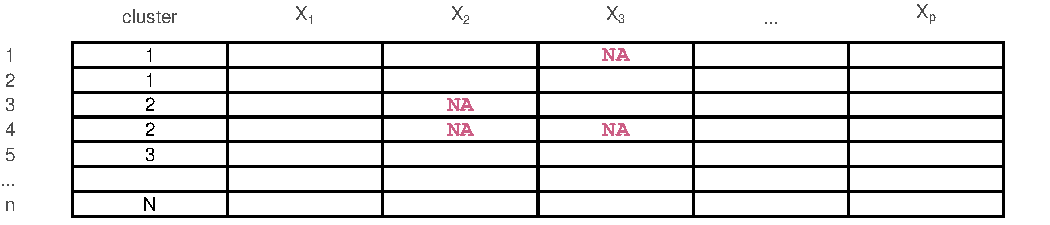
\includegraphics{manuscript_files/figure-pdf/unnamed-chunk-3-1.pdf}

}

\end{figure}

Column \(X_1\) in Figure 1 is completely observed, column \(X_2\) is
systematically missing in cluster 2, and column \(X_3\) is sporadically
missing. To analyze these incomplete data, we have to take the nature of
the missingness and the cluster structure into account. For example, the
sporadic missingness in \(X_3\) could be easily amended if this would be
a cluster-level variable (and thus constant within clusters). We could
then just extrapolate the true (but missing) value of \(X_3\) for unit 1
from unit 2, and the value for unit 4 from unit 3. If \(X_3\) would
instead be a unit-level variable (which may vary within clusters), we
could not just recover the unobserved `truth', but would need to use
some kind of missing data method, or discard the incomplete units
altogether (i.e., complete case analysis). Complete case analysis can
however introduce bias in statistical inferences and lowers statistical
power. Further, with the systematic missingness in \(X_2\), it would be
impossible to fit a multilevel model without accommodating the
missingness in some way. Complete case analysis in that case would mean
excluding the entire cluster from the analyses. The wrong choice of
missing data handling method can thus be extremely harmful to the
inferences.

Imputation of missing data requires consideration of the mechanism
behind the missingness. Rubin proposed to distinguish between data that
are missing completely at random (MCAR), data that are missing at random
(MAR) and data that are missing not at random (MNAR; see Table
\ref{tab:miss}). For each of these three missingness generating
mechanisms, different imputation strategies are warranted
(\citet{yuce08} and \citet{hox15}). We here consider the general case
that data are MAR, and expand on certain MNAR situations.

\hypertarget{imputation-with-mice}{%
\subsection{imputation with mice}\label{imputation-with-mice}}

The \proglang{R} package \pkg{mice} provides a framework for imputing
incomplete data on a variable-by-variable basis. The \fct{mice} function
allows users to flexibly specify how many times and under what model the
missing data should be imputed. This is reflected in the first four
function arguments

\begin{verbatim}
mice(data, m, method, predictorMatrix, ...)
\end{verbatim}

where \texttt{data} refers to the incomplete dataset, \texttt{m}
determines the number of imputations, \texttt{method} denotes the
functional form of the imputation model and \texttt{predictorMatrix}
specifies the interrelational dependencies between variables and
imputation models (i.e., the set of predictors to be used for imputing
each incomplete variable).

\begin{tcolorbox}[enhanced jigsaw, toprule=.15mm, arc=.35mm, rightrule=.15mm, breakable, opacityback=0, bottomrule=.15mm, colback=white, leftrule=.75mm, left=2mm]

Box 2. The \texttt{methods}.

\end{tcolorbox}

\begin{tcolorbox}[enhanced jigsaw, toprule=.15mm, arc=.35mm, rightrule=.15mm, breakable, opacityback=0, bottomrule=.15mm, colback=white, leftrule=.75mm, left=2mm]

Box 3. The predictor matrix. The entries corresponding to the level-1
predictors are coded with a 3, indicating that both the original values
as well as the cluster means of the predictor are included into the
imputation model. The entry of 4 in the predictor matrix adds three
variables to the imputation model for the imputation model predictor:
the value of the predictor, the cluster means of the predictor and the
random slopes of the predictor. - -2 = cluster variable - 1 = overall
effect - 3 = overall + group-level effect - 4 = individual-level
(random) and group-level (fixed) effect

\end{tcolorbox}

\hypertarget{sec-workflow}{%
\section{Multilevel imputation workflow}\label{sec-workflow}}

There are different strategies that can be adopted in the imputation
process that account for clustering: inclusion of cluster indicator
variable, performing a separate imputation process for each cluster, or
performing a simultaneous imputation process by using an imputation
method that accounts for clustering.(Stata:
https://www.stata.com/support/faqs/statistics/clustering-and-mi-impute/)
TODO: replace ref.

The selection of each strategy depends mainly on the assumptions in the
main analysis and also on the restriction of the analyzed data.

Regarding the restrictions imposed by the data, for instance, the use of
cluster indicator variables is restricted in datasets where there are
not many clusters and many observations per cluster (Graham, 2009). The
last restriction is also required when imputations are performed on each
cluster separately. When this restriction cannot be achieved, one can
use an imputation model that simultaneously imputes all clusters using a
hierarchical model (Allison 2002).

Under this hierarchical imputation model, observations within clusters
are correlated and this correlation is modeled by a random effect so the
hierarchical model can be estimated even when there are few observations
per cluster. However, this strategy is best suited for balanced data
(Grund, 2017) and when random effects model is appropriated, i.e.~the
number of clusters is adequate. (Austin,2018).

Here it is important to evaluate the assumptions imposed by the main
model, for instance by using the cluster indicator strategy may lead to
bias estimates when the model is based on a hierarchical model
(Taaljard,2008). Even when an imputation strategy congenial with the
main model is preferred, it is important to consider whether it is
appropriate for the data as a less complex imputation strategies may
also lead to unbiased estimates in certain scenarios(Bailey 2020). For
instance, in causal effect analysis, separately imputation may lead to
smaller bias when the size of the smaller exposure cluster is large,
compared with an imputation model that includes exposure-confounder
interactions. (Zhang,2023).

Below we provide a imputation workflow that can be used in general to
impute cluster data.

\hypertarget{focus-on-the-main-analysis}{%
\subsection{Focus on the Main
Analysis}\label{focus-on-the-main-analysis}}

When dealing with incomplete clustered data, start by looking at your
research questions and planned analysis. Pretend there are no missing
data at first. This will help you understand your research hypotheses,
the main statistical model, and give you insights into your data's
structure (refer to the level table), variable types (e.g., confounders,
auxiliary variables), and other considerations such as variable
relationships, interactions or polynomial terms.

\hypertarget{exploration-of-available-data}{%
\subsection{Exploration of Available
Data}\label{exploration-of-available-data}}

Now, explore what's in your data. Use simple tools like histograms and
QQ plots to understand variable distributions, plausible range of values
and identify errors or outliers. Check interactions between predictors
with scatter plots, look for collinearity with VIF or correlations
plots, this may also help you to identify non-considered relationships
that may affect the main model. You might also consider to test
assumptions related to your response variable such as variance
homogeneity, independence between observations (eg. ACF, variagrams).
This will help you choose an imputation model that suits your data. In
addition, the intraclass correlation coefficient (ICC) can be examined
to assess cluster differences, aiding in the choice between the 2l and
1l methods for imputation.

Next, explore the missingness. Look at the
\textbf{proportion of missing values} in the dataset variables. This
helps find potential predictors and cut down on unnecessary variables in
the imputation model. Doing this can lower the risk of multicollinearity
or computational issues, especially with certain parametric imputation
methods. You can also identify predictors for the imputation model by
using inflow criteria to see connections between missing data in one
variable and observed variables, and outflow criteria to identify
connections between observed values in one variable and missing data in
others.

Check the missing patterns at cluster level, this can help you to select
the most appropiated imputation approach in terms of computational
efficiency (e.g., simpler regression imputation versus FCS in univariate
patterns).

\hypertarget{assess-estimation-procedure-robustness-to-missing-data}{%
\subsection{Assess Estimation Procedure Robustness to Missing
Data}\label{assess-estimation-procedure-robustness-to-missing-data}}

Before diving into imputation, make sure your estimation model can
handle missing data. Sometimes, simpler methods like complete case
analysis might be suffice, especially if your missingness is low
(usually \textless5\%). There are scenarios in which specific Maximum
Likelihood (ML) estimation methods outperform Multiple Imputation (MI)
methods, for instance when the response variable is the sole incomplete
variable, mixed models demonstrate robustness to missing data under the
Missing at Random (MAR) assumption and with a correct
variance-covariance specification.\cite{Molenberghs_2007}.

\hypertarget{pre-imputation}{%
\subsection{Pre-imputation}\label{pre-imputation}}

Clean up your dataset before the imputation process. Keep initially the
essential variables for your main model, but include extra variables if
needed for specific procedures during analysis (e.g.~confounders on
balancing procedures). Think about adding other useful variables, even
if they're not in the main model, such as instrumental or auxiliary
variables which might boost your parameter estimates, especially if
they're associated to the probability of missingness for some incomplete
variables.

Figure out if you can directly impute incomplete variables by just use
deductive imputation. This involves inferring missing values based on
logicallogical connections between variables. It's especially handy for
variables that depend on each other, like calculating BMI from weight
and height.

Deductive imputation is also useful for getting values for level-1
variables from level-2 ones, like in Individual Participant Data (IPD).
In these situations, you can guess missing information from metadata or
by using or through deduction based on time or protocols. For example,
you could deduce missing test values for patients who have passed away.

\hypertarget{setting-imputation-model}{%
\subsection{Setting Imputation Model}\label{setting-imputation-model}}

\hypertarget{clustering-inclusion}{%
\paragraph{Clustering Inclusion}\label{clustering-inclusion}}

When it comes to handling clusters during the imputation process, you've
got a few options. You can use a cluster indicator variable, run
separate imputation for each cluster, or go for a simultaneous
imputation method that takes clustering into account \cite{eddings}.

Which strategy you choose depends on the assumptions in your main
analysis and the limitations of your data. If your analysis do not use a
hierarchical model (like a descriptive approach) and you have a small
number of clusters with lots of observations in each, using a cluster
indicator or separate imputation might be the way to go
\cite{graham2009}. Conversely, if you have more clusters or fewer
observations per cluster, you might want to try a simultaneous
hierarchical imputation model \cite{Allison_2002}.

In a hierarchical imputation model, random effects model the
correlations between observations within clusters, making it possible to
estimate even with a small number of observations per cluster. There are
various proposed multiple imputation models based on hierarchical
models, each with its own set of assumptions \cite{audigier}.

If your analysis uses a hierarchical model, make sure the assumptions of
your imputation model match up. For example, using a cluster indicator
approach may lead to bias estimates if your model is based on a
hierarchical structure \cite{taljaard2008,speidel2018}. Even if you
prefer an imputation strategy that aligns with your main model, check if
it suits your data; sometimes simpler strategies can give unbiased
estimates in certain scenarios \cite{bailey2020}.

\hypertarget{choice-of-individual-imputation-methods}{%
\subsubsection{Choice of Individual Imputation
Methods}\label{choice-of-individual-imputation-methods}}

Start by choosing the imputation model for each incomplete variable in
your dataset. The mice package suggests methods based on variable types
for non-clustered variables, and for the cluster ones, you can use the
micemd package's find.defaultMethod() function. This function selects
from different 2l imputation methods based on cluster size and the
proportion of missing data in each cluster.

Besides the package-defined imputation methods, you can specify custom
methods using the ``I formula''. This lets you calculate deterministic
variables during the imputation or tweak imputation methods based on
specific conditions, like conditioning the imputation model to the level
of an incomplete covariate (e.g., a pregnancy test for females).

\hypertarget{model-specification}{%
\subsubsection{Model Specification}\label{model-specification}}

The imputation model must be congenial with the main model
\cite{meng1994}. Congeniality issues arise when the imputation model and
the main model make different assumptions, often due to the omission of
a polynomial or interaction term or the use of transformed variables.

The imputation model can incorporate additional terms compared to the
main model without causing compatibility issues. For instance, it's
recommended to include the outcome variable in the imputation model for
prediction variables \cite{moons2006a}. In cases where the outcome is
time-to-event, the Nelson-Aalen estimate of the time to the event should
be added as a covariate in the imputation model {[}REF{]}. Additionally,
including auxiliary variables, even if not part of the main model, can
be linked to the probability of missingness, improving the likelihood of
meeting the Missing at Random (MAR) assumption and enhancing estimation
efficiency \cite{hardt2012a}.

Imputation models are specified on a variable basis, either using a
prediction matrix in the pred parameter or through a list of formulas in
the formula parameter. In the prediction matrix option, the type of each
predictor variable is specified for each incomplete variable (see
table).

\begin{align}
y_{ij} =& (\beta_0 + b_{0_i})+ \beta_1x_{1_{ij}}+\beta_2x_{2_{i.}} \nonumber \\
+& (\beta_3 +  b_{3_i})x_{3_{ij}} \nonumber \\
+& \beta_4x_{4_{ij}} + \beta_{m4}\overline{x_{4_{i.}}}\nonumber \\
+& (\beta_5 +  b_{5_i})x_{5_{ij}} +\beta_{m5}\overline{x_{5_{i.}}}\nonumber \\
\end{align}

\begin{tabular}{ll}
     \toprule
Type & Definition \\
  \midrule
-2  & Cluster variable, in this case the one defined by j index  \\
 1  & Fixed variable, e.g., level-1  $x_{1_{ij}}$ or  level-2 $x_{2_{i.}}$ \\
 2  & Random variable, e.g., $x_{3_{ij}}$\\
 3  & *Fixed variable with cluster mean $x_{4_{ij}}$\\
 4  & *Random variable with cluster mean $x_{5_{ij}}$\\
-3. & Random variable only included on selection model (Heckman model)\\
-4. & Random variable only included on main model (Heckman model)\\
      \bottomrule
\end{tabular}

\begin{itemize}
\tightlist
\item
  3 and 4 type have been advised to used as the inclusion of the means
  of the cluster is beneficial on FCS \cite{mistler2017}
\end{itemize}

Recipes have been proposed for imputing incomplete level-1 and level-2
variables for hierarchical models \cite{buuren2018a} (\(\S\) 7.10),
which can be convenient to follow when dealing with numerous variables
(interaction terms at different levels) and models with many random
effects that are prone to convergency problems due to overspecification
in the imputation model. These rules were designed to ensure
compatibility among the conditionally specified imputation models and
congeniality between the imputation and the main model. However, they
may not be applicable to all 2l imputation methods; for instance, the
2l.2stage imputation methods of the micemd package only allow the
inclusion of random predictor variables (2).

On the other hand, the formula option is useful in specifying complex
imputation models with polynomial terms or interactions and compared
with the prediction matrix method do not requires the inclusion of
additional terms as Just Another Variable (JAV)
\cite{buuren2018a}(\(\S\) 6.4).

For some interaction terms, it has been suggested, for instance, for
treatment interaction effects, to conduct separate imputation by
treatment group \cite{zhang2023}. Additionally, it can be used
imputation models based on random forest or deep learning that can
handle interaction and non-linear terms without requiring the explicit
specification of an imputation model.

\hypertarget{post-imputation}{%
\subsection{Post-Imputation}\label{post-imputation}}

During the imputation process, certain issues may arise that halt the
process. In hierarchical model imputations, many issues are related to
over fitting the imputation model. To troubleshoot, it is recommended to
inspect the imputation log file for variables causing problems. One
approach to address this is to reduce the number of predictors, by using
step by step the previous referred recepies or by using functions like
quickpred. Another option is to consider variable transformations, such
as scaling when model is invariant to linear transformations e.g.,
random intercept models. Also adjusting the level of the hierarchical
model (e.g., using a homogeneous variance imputation method or a 1l
model) can also be beneficial.

It is crucial to check the range of imputed variables, as excessively
large imputed values for one predictor may trigger convergence issues in
other variables. To tackle this, including post-processing
specifications on problematic variables or utilizing imputation models
like Predicted Mean Matching (PMM) can ensure that imputed values align
with observable values.

In some situations, adopting a separate imputation strategy might be
worth considering. For example, in analyses involving multiple
endpoints, conducting distinct imputation processes for each endpoint
could be more effective than a unified imputation approach.

\hypertarget{convergence-and-sensitivity-analysis}{%
\subsection{Convergence and Sensitivity
Analysis}\label{convergence-and-sensitivity-analysis}}

Before starting into the analysis of each imputed dataset, it is crucial
to validate the convergence of the imputation process. This is commonly
accomplished through trace plots that depict the mean and variance of
the incomplete variables across iterations. These plots serve to uncover
potential circular issues or the need for additional iterations.
Additionally, it is also important to verify that imputed values fall
within a plausible range and also to check the distribution of imputed
variables, ensuring that the imputed variable distribution aligns with
the distribution of observed values (under the MAR assumption). An
alternative approach involves assessing the prediction accuracy of the
imputation method \cite{cai2023}.

While the majority of Multiple Imputation by Chained Equations (MICE)
methods are based on Missing at Random (MAR) assumptions, field expert
input may suggest that the Missing Not at Random (MNAR) mechanism could
be plausible for certain variables. An MNAR variable is one in which the
probability of missingness depends on an unobservable variable. This can
occur when missingness is associated with the incomplete value itself
(self-marking) or when there is an unobserved variable linked to both
the value and the probability of missingness of the incomplete value
(indirectly non-informative). Specifically, for the indirectly
non-informative case in hierarchical datasets, imputation methods based
on the Heckman method can be
considered.\cite{hammon2020,hammon2022,munoz2023}

\begin{center}\rule{0.5\linewidth}{0.5pt}\end{center}

\hypertarget{sec-illustrations}{%
\section{Illustrations}\label{sec-illustrations}}

In this section, we demonstrate the workflow using three case studies.

\hypertarget{setup}{%
\subsection{Setup}\label{setup}}

\begin{verbatim}
R> set.seed(123)         # for reproducibility
R> library(lme4)         # for multilevel modeling
R> library(nlme)         # for multilevel modeling
R> library(mice)         # for imputation
R> library(miceadds)     # for multilevel imputation methods
R> library(micemd)       # for selection-model imputation methods
R> library(mitml)        # for multilevel parameter pooling
R> library(broom)        # for clean model estimates
R> library(broom.mixed)  # for multilevel model estimates
R> library(dplyr)        # for data wrangling
R> library(ggmice)       # for visualization
R> library(ggplot2)      # for visualization
\end{verbatim}

\hypertarget{popularity-data}{%
\subsection{Popularity data}\label{popularity-data}}

In this section we will go over the different steps involved with
imputing incomplete multilevel data with the R package mice. We consider
the simulated \texttt{popmis} dataset, which included pupils
(\(n = 2000\)) clustered within schools (\(N = 100\)). The following
variables are of primary interest:

\begin{itemize}
\tightlist
\item
  \texttt{school}, school identification number (clustering variable);
\item
  \texttt{popular}, pupil popularity (self-rating between 0 and 10;
  unit-level);
\item
  \texttt{sex}, pupil sex (0 = boy, 1 = girl; unit-level);
\item
  \texttt{texp}, teacher experience (in years; cluster-level).
\end{itemize}

The analysis model corresponding to this dataset is multilevel
regression with random intercepts for the different schools. We will
estimate the association between the pupils' sex and their popularity
score. This model can be expressed in \texttt{lme4} code as:

\begin{verbatim}
popular ~ 1 + sex + (1 | school)
\end{verbatim}

Given the \(j\)-th student belonging to the \(i\)-th school, the main
model can be formulated as:

\[ popular_{ij} = (\beta_0 + b_i) + \beta_1sex_{ij}+ \beta_2texp_{ij}+\epsilon_{ij}\]
where \(\epsilon_{ij}\) corresponds to the error term.

We load the data into the environment with

\begin{verbatim}
R> data("popmis", package = "mice")
\end{verbatim}

and select the relevant variables

\begin{verbatim}
R> dat <- popmis[, c("school", "popular", "texp", "sex")] 
\end{verbatim}

which results in the following data structure.

\begin{verbatim}
R> head(dat)
\end{verbatim}

\begin{verbatim}
  school popular texp sex
1      1      NA   24   1
2      1      NA   24   0
3      1       7   24   1
4      1      NA   24   1
5      1      NA   24   1
6      1       7   24   0
\end{verbatim}

The association of interest can be visualized with \texttt{ggmice},

\begin{verbatim}
ggmice(dat, aes(sex, popular)) +
  geom_jitter()
\end{verbatim}

\begin{figure}[h]

{\centering 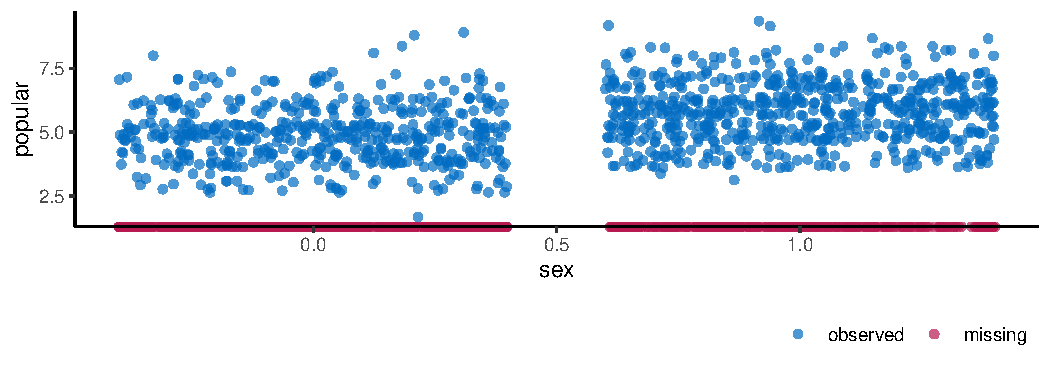
\includegraphics{manuscript_files/figure-pdf/unnamed-chunk-8-1.pdf}

}

\caption{Scatterplot of student popularity by sex}

\end{figure}

where missing datapoints in the \texttt{popular} variable are
represented by red points on the X-axis of the figure.

With the \texttt{ggmice} function \texttt{plot\_pattern} we can
visualize the missing data pattern

\begin{verbatim}
R> plot_pattern(dat)
\end{verbatim}

\begin{figure}[h]

{\centering 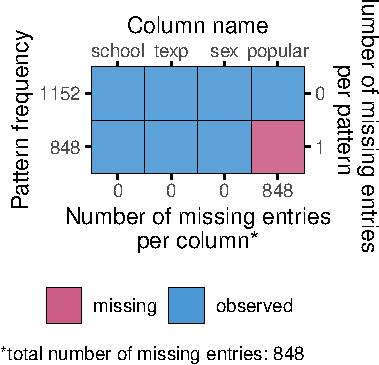
\includegraphics{manuscript_files/figure-pdf/fig-pattern-1.pdf}

}

\caption{\label{fig-pattern}Missing data pattern.}

\end{figure}

which shows us that the missingness is univariate and sporadic.

To develop the best imputation model for the incomplete variable
\texttt{popular}, we need to know whether the observed values of
\texttt{popular} are related to observed values of other variables. Plot
the pair-wise complete correlations in the incomplete data

\begin{verbatim}
R> plot_corr(dat)
\end{verbatim}

\begin{figure}[h]

{\centering 
\includegraphics{manuscript_files/figure-pdf/unnamed-chunk-10-1.pdf}

}

\caption{Pair-wise correlations.}

\end{figure}

This shows us that not just the analysis-model variable \texttt{sex},
but also the cluster-level covariate teacher experience, \texttt{texp},
may be a useful as an imputation model predictor. Moreover, the
missingness in \texttt{popular} may depend on the observed values of
other variables. With \texttt{ggmice()} we can visualize the
distribution of the teacher experience for cases where \texttt{popular}
is observed and cases where \texttt{popular} is missing.

\begin{verbatim}
R> ggmice(dat, aes(texp)) + 
+  geom_density() +
+  facet_wrap(~is.na(popular))
\end{verbatim}

\begin{figure}[h]

{\centering 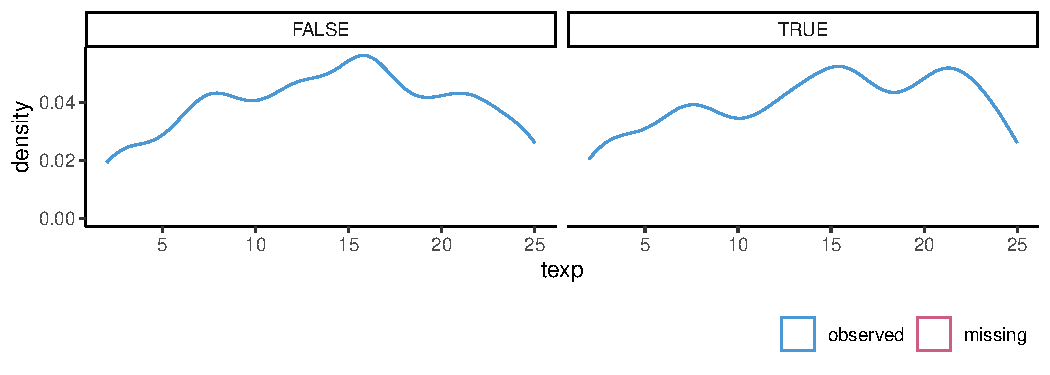
\includegraphics{manuscript_files/figure-pdf/unnamed-chunk-11-1.pdf}

}

\end{figure}

It appears that students with a missing value for \texttt{popular} are
in clusters with a slightly higher \texttt{texp} value.

\begin{verbatim}
t.test(dat$texp ~ is.na(dat$popular)) |> 
  tidy() |>
  kable()
\end{verbatim}

\begin{longtable}[]{@{}
  >{\raggedleft\arraybackslash}p{(\columnwidth - 18\tabcolsep) * \real{0.0924}}
  >{\raggedleft\arraybackslash}p{(\columnwidth - 18\tabcolsep) * \real{0.0840}}
  >{\raggedleft\arraybackslash}p{(\columnwidth - 18\tabcolsep) * \real{0.0840}}
  >{\raggedleft\arraybackslash}p{(\columnwidth - 18\tabcolsep) * \real{0.0924}}
  >{\raggedleft\arraybackslash}p{(\columnwidth - 18\tabcolsep) * \real{0.0840}}
  >{\raggedleft\arraybackslash}p{(\columnwidth - 18\tabcolsep) * \real{0.0840}}
  >{\raggedleft\arraybackslash}p{(\columnwidth - 18\tabcolsep) * \real{0.0924}}
  >{\raggedleft\arraybackslash}p{(\columnwidth - 18\tabcolsep) * \real{0.0840}}
  >{\raggedright\arraybackslash}p{(\columnwidth - 18\tabcolsep) * \real{0.2017}}
  >{\raggedright\arraybackslash}p{(\columnwidth - 18\tabcolsep) * \real{0.1008}}@{}}
\toprule\noalign{}
\begin{minipage}[b]{\linewidth}\raggedleft
estimate
\end{minipage} & \begin{minipage}[b]{\linewidth}\raggedleft
estimate1
\end{minipage} & \begin{minipage}[b]{\linewidth}\raggedleft
estimate2
\end{minipage} & \begin{minipage}[b]{\linewidth}\raggedleft
statistic
\end{minipage} & \begin{minipage}[b]{\linewidth}\raggedleft
p.value
\end{minipage} & \begin{minipage}[b]{\linewidth}\raggedleft
parameter
\end{minipage} & \begin{minipage}[b]{\linewidth}\raggedleft
conf.low
\end{minipage} & \begin{minipage}[b]{\linewidth}\raggedleft
conf.high
\end{minipage} & \begin{minipage}[b]{\linewidth}\raggedright
method
\end{minipage} & \begin{minipage}[b]{\linewidth}\raggedright
alternative
\end{minipage} \\
\midrule\noalign{}
\endhead
\bottomrule\noalign{}
\endlastfoot
-0.2599581 & 14.15278 & 14.41274 & -0.8731291 & 0.3827095 & 1796.115 &
-0.8438947 & 0.3239786 & Welch Two Sample t-test & two.sided \\
\end{longtable}

Although there are no significant differences in the distribution of
\texttt{texp} depending on the missingness indicator of
\texttt{popular}, this variable can serve as auxiliary variable in the
imputation of \texttt{popular}.

\begin{verbatim}
R> meth <- make.method(dat)
R> meth
\end{verbatim}

\begin{verbatim}
 school popular    texp     sex 
     ""   "pmm"      ""      "" 
\end{verbatim}

\begin{verbatim}
R> pred <- quickpred(dat)
R> pred
\end{verbatim}

\begin{verbatim}
        school popular texp sex
school       0       0    0   0
popular      0       0    1   1
texp         0       0    0   0
sex          0       0    0   0
\end{verbatim}

Adjust the methods vector.

\begin{verbatim}
R> meth["popular"] <- "2l.pmm"
\end{verbatim}

The \texttt{pmm} method is better (more efficient) because it will still
look for donors (maybe outside of cluster) based on predictive distance,
even for very small clusters.

Adjust the predictor matrix.

\begin{verbatim}
R> pred["popular", "school"] <- -2
R> pred["popular", "sex"] <- 2
\end{verbatim}

Visualize the imputation methods and predictors.

\begin{verbatim}
plot_pred(pred, method = meth)
\end{verbatim}

\begin{figure}[h]

{\centering 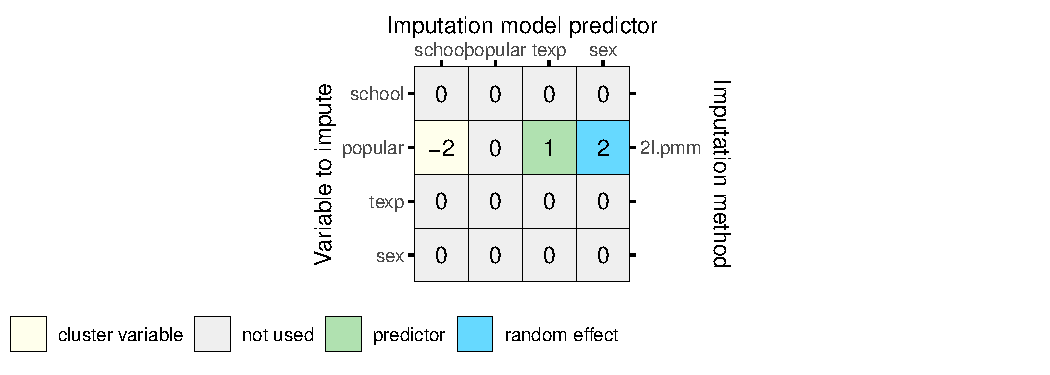
\includegraphics{manuscript_files/figure-pdf/unnamed-chunk-17-1.pdf}

}

\end{figure}

Impute the data.

\begin{verbatim}
R> imp <- mice(
+  data = dat,
+  method = meth,
+  predictorMatrix = pred,
+  printFlag = FALSE
+)
\end{verbatim}

Evaluate the convergence.

\begin{verbatim}
R> plot_trace(imp)
\end{verbatim}

\begin{figure}[h]

{\centering 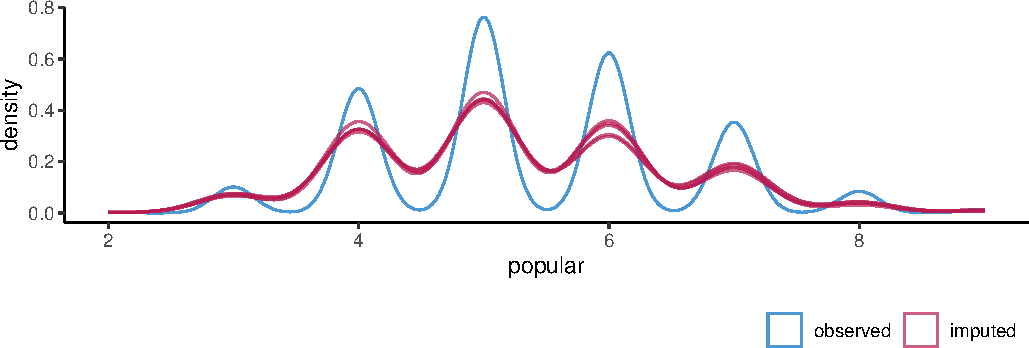
\includegraphics{manuscript_files/figure-pdf/unnamed-chunk-19-1.pdf}

}

\end{figure}

Troubleshoot non-convergence of imputation model. Evaluate the
distribution of imputed values.

\begin{verbatim}
R> ggmice(imp, aes(popular, group = .imp)) + 
+  geom_density() 
\end{verbatim}

\begin{figure}[h]

{\centering 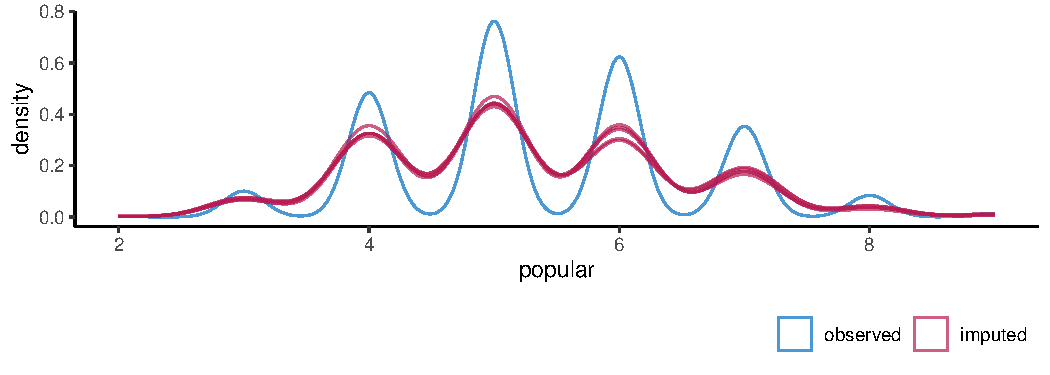
\includegraphics{manuscript_files/figure-pdf/unnamed-chunk-20-1.pdf}

}

\end{figure}

Evaluate the distribution of imputed values.

\begin{verbatim}
R> ggmice(imp, aes(.imp, popular)) + 
+  geom_jitter(alpha = 0.05) +
+    geom_boxplot()
\end{verbatim}

\begin{figure}[h]

{\centering 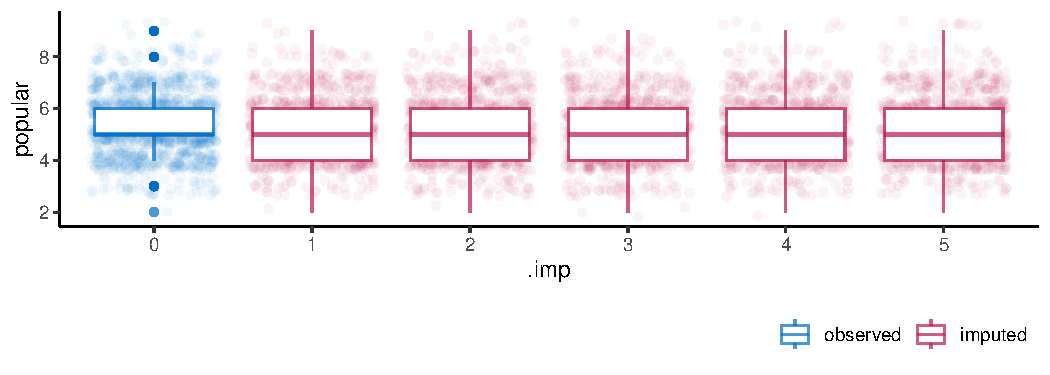
\includegraphics{manuscript_files/figure-pdf/unnamed-chunk-21-1.pdf}

}

\end{figure}

\begin{verbatim}
R> ggmice(imp, aes(sex, popular)) +
+  geom_jitter() +
+  facet_wrap(~ .imp)
\end{verbatim}

\begin{figure}[h]

{\centering 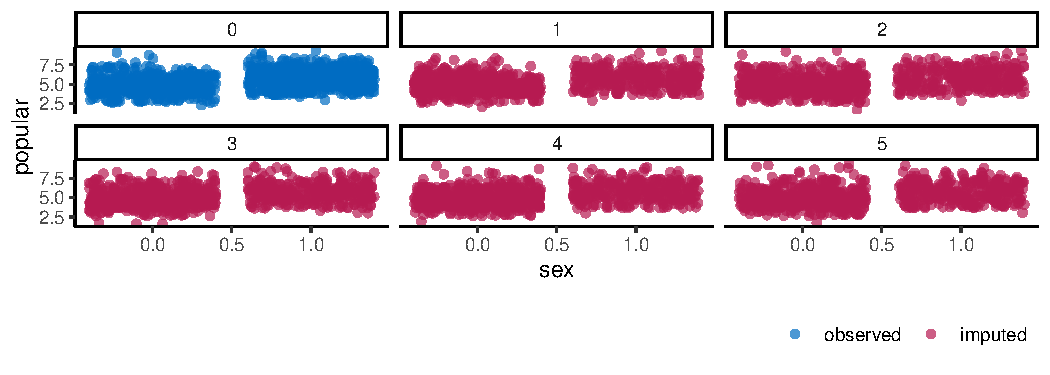
\includegraphics{manuscript_files/figure-pdf/unnamed-chunk-22-1.pdf}

}

\end{figure}

Analyze the imputed data.

\begin{verbatim}
R> fit <- with(
+  imp,
+  lmer(popular ~ texp + sex + (1 | school))
+)
\end{verbatim}

Pooling the estimates does not provide estimates of the variance
components.

\begin{verbatim}
R> pool(fit)
\end{verbatim}

\begin{verbatim}
Class: mipo    m = 5 
         term m   estimate         ubar            b            t dfcom
1 (Intercept) 5 3.59902513 0.0284760238 3.461284e-03 0.0326295651  1995
2        texp 5 0.09225928 0.0001140591 2.273382e-05 0.0001413397  1995
3         sex 5 0.85187018 0.0009628869 4.946825e-04 0.0015565060  1995
        df       riv    lambda       fmi
1 216.1756 0.1458610 0.1272938 0.1352573
2 100.6502 0.2391794 0.1930144 0.2085857
3  26.9008 0.6164992 0.3813792 0.4227574
\end{verbatim}

Therefore, \texttt{mitml} is used.

\begin{verbatim}
R> est <- testEstimates(as.mitml.result(fit), extra.pars = TRUE)
\end{verbatim}

Display results in table.

\begin{verbatim}
R> est$estimates |> 
+  round(3) |>
+  kable()
\end{verbatim}

\begin{longtable}[]{@{}
  >{\raggedright\arraybackslash}p{(\columnwidth - 14\tabcolsep) * \real{0.1558}}
  >{\raggedleft\arraybackslash}p{(\columnwidth - 14\tabcolsep) * \real{0.1169}}
  >{\raggedleft\arraybackslash}p{(\columnwidth - 14\tabcolsep) * \real{0.1299}}
  >{\raggedleft\arraybackslash}p{(\columnwidth - 14\tabcolsep) * \real{0.1039}}
  >{\raggedleft\arraybackslash}p{(\columnwidth - 14\tabcolsep) * \real{0.1039}}
  >{\raggedleft\arraybackslash}p{(\columnwidth - 14\tabcolsep) * \real{0.2338}}
  >{\raggedleft\arraybackslash}p{(\columnwidth - 14\tabcolsep) * \real{0.0779}}
  >{\raggedleft\arraybackslash}p{(\columnwidth - 14\tabcolsep) * \real{0.0779}}@{}}
\toprule\noalign{}
\begin{minipage}[b]{\linewidth}\raggedright
\end{minipage} & \begin{minipage}[b]{\linewidth}\raggedleft
Estimate
\end{minipage} & \begin{minipage}[b]{\linewidth}\raggedleft
Std.Error
\end{minipage} & \begin{minipage}[b]{\linewidth}\raggedleft
t.value
\end{minipage} & \begin{minipage}[b]{\linewidth}\raggedleft
df
\end{minipage} & \begin{minipage}[b]{\linewidth}\raggedleft
P(\textgreater\textbar t\textbar)
\end{minipage} & \begin{minipage}[b]{\linewidth}\raggedleft
RIV
\end{minipage} & \begin{minipage}[b]{\linewidth}\raggedleft
FMI
\end{minipage} \\
\midrule\noalign{}
\endhead
\bottomrule\noalign{}
\endlastfoot
(Intercept) & 3.599 & 0.181 & 19.924 & 246.857 & 0 & 0.146 & 0.134 \\
texp & 0.092 & 0.012 & 7.760 & 107.369 & 0 & 0.239 & 0.208 \\
sex & 0.852 & 0.039 & 21.592 & 27.501 & 0 & 0.616 & 0.422 \\
\end{longtable}

\begin{verbatim}
R> est$extra.pars |> 
+  round(3) |>
+  kable()
\end{verbatim}

\begin{longtable}[]{@{}lr@{}}
\toprule\noalign{}
& Estimate \\
\midrule\noalign{}
\endhead
\bottomrule\noalign{}
\endlastfoot
Intercept\textasciitilde\textasciitilde Intercept\textbar school &
0.470 \\
Residual\textasciitilde\textasciitilde Residual & 0.462 \\
ICC\textbar school & 0.504 \\
\end{longtable}

\hypertarget{impact-data}{%
\subsection{IMPACT data}\label{impact-data}}

The second case study is the \texttt{impact} data from the
\pkg{metamisc} package \citep[empirical data on traumatic brain
injuries, \(n = 11,022\) units across \(N = 15\) clusters,][]{metamisc}.

The \texttt{impact} data set contains traumatic brain injury data on
\(n = 11022\) patients clustered in \(N = 15\) studies with the
following 11 variables:

\begin{itemize}
\tightlist
\item
  \texttt{name} Name of the study,
\item
  \texttt{type} Type of study (RCT: randomized controlled trial, OBS:
  observational cohort),
\item
  \texttt{age} Age of the patient,
\item
  \texttt{motor\_score} Glasgow Coma Scale motor score,
\item
  \texttt{pupil} Pupillary reactivity,
\item
  \texttt{ct} Marshall Computerized Tomography classification,
\item
  \texttt{hypox} Hypoxia (0=no, 1=yes),
\item
  \texttt{hypots} Hypotension (0=no, 1=yes),
\item
  \texttt{tsah} Traumatic subarachnoid hemorrhage (0=no, 1=yes),
\item
  \texttt{edh} Epidural hematoma (0=no, 1=yes),
\item
  \texttt{mort} 6-month mortality (0=alive, 1=dead).
\end{itemize}

Check if there is systematic missingness in this dataset. For
illustration purposes, we made Marshall Computerized Tomography
classification (ct) systematically missing.

The analysis model for this dataset is a prediction model with
\texttt{mort} as the outcome. In this tutorial we'll estimate the
adjusted prognostic effect of \texttt{ct} on mortality outcomes. The
estimand is the adjusted odds ratio for \texttt{ct}, after including
\texttt{type}, \texttt{age} \texttt{motor\_score} and \texttt{pupil}
into the analysis model:

\begin{verbatim}
mort ~ type + age + motor_score + pupil + ct + (1 | name) 
\end{verbatim}

In this dataset all the variables are level-1 (patient), except by the
level-2 (study) type variable. The analysis model for this dataset is a
prediction model with \texttt{mort} as the outcome. In this tutorial
we'll estimate the adjusted prognostic effect of \texttt{ct} on
mortality outcomes. The estimand is the adjusted odds ratio for
\texttt{ct}, after including \texttt{type}, \texttt{age}
\texttt{motor\_score} and \texttt{pupil}. Therefore the main model for
the \(i\)-th patient from the \(j\)-th study can be described as:

\[ mort_{ij} = (\beta_0 + b_i) + \beta_1type_{.j}+ \beta_2age_{ij}+ \beta_3motorscore_{ij} + \beta_4pupil_{ij} + \beta_5ct_{ij}+\epsilon_{ij}\]
where \(\epsilon_{ij}\) corresponds to the error term.

Note that variables \texttt{hypots}, \texttt{hypox}, \texttt{tsah} and
\texttt{edh} are not part of the analysis model, and may thus serve as
auxiliary variables for imputation.

The \texttt{impact} data included in the \pkg{metamisc} package is a
complete data set. The original data has already been imputed once
(Steyerberg et al, 2008). For the purpose of this tutorial we have
induced missingness (mimicking the missing data in the original data set
before imputation). The resulting incomplete data can be accessed from
\href{https://zenodo.com}{zenodo link to be created}.

Load the incomplete data into the R workspace:

\begin{verbatim}
R> dat <- read.table("link/to/the/data.txt") 
\end{verbatim}

To explore the missingness, we should look at the missing data pattern.
The ten most frequent missingness patterns are shown with

\begin{verbatim}
R> plot_pattern(dat, rotate = TRUE, npat = 10L)  
\end{verbatim}

\begin{figure}[h]

{\centering 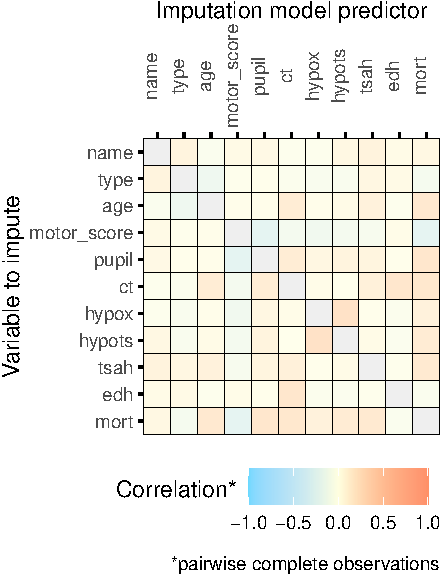
\includegraphics{manuscript_files/figure-pdf/unnamed-chunk-28-1.pdf}

}

\end{figure}

This shows that we need to impute \texttt{ct} and \texttt{pupil}. To
develop the best imputation model, we need to investigate the relations
between the observed values of the incomplete variables and the observed
values of other variables, and the relation between the missingness
indicators of the incomplete variables and the observed values of the
other variables. To see whether the missingness depends on the observed
values of other variables, we can test this statistically or use visual
inspection (e.g.~a histogram faceted by the missingness indicator).

We should impute the variables \texttt{ct} and \texttt{pupil} and any
auxiliary variables we might want to use to impute these incomplete
analysis model variables. We can evaluate which variables may be useful
auxiliaries by plotting the pairwise complete correlations

\begin{verbatim}
R> plot_corr(dat, rotate = TRUE)
\end{verbatim}

\begin{figure}[h]

{\centering 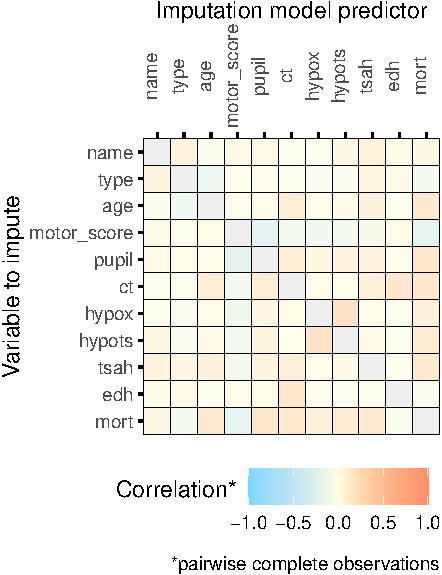
\includegraphics{manuscript_files/figure-pdf/unnamed-chunk-29-1.pdf}

}

\end{figure}

This shows us that \texttt{hypox} and \texttt{hypot} would not be useful
auxiliary variables for imputing \texttt{ct}. Depending on the minimum
required correlation, \texttt{tsah} could be useful, while \texttt{edh}
has the strongest correlation with \texttt{ct} out of all the variables
in the data and should definitely be included in the imputation model.
For the imputation of \texttt{pupil}, none of the potential auxiliary
variables has a very strong relation, but \texttt{hypots} could be used.
We conclude that we can exclude \texttt{hypox} from the data, since this
is neither an analysis model variable nor an auxiliary variable for
imputation

\begin{verbatim}
R> dat <- select(dat, !hypox)
\end{verbatim}

Mutate data to get the right data types for imputation (e.g.~integer for
clustering variable).

\begin{verbatim}
R> # dat <- mutate(
R> #   dat,
R> #   name = as.integer(name))
\end{verbatim}

This is necessary because otherwise PMM cannot be used for these factor
variables.

\begin{verbatim}
R> dat <- mutate(
+  dat,
+  across(everything(), as.numeric))
\end{verbatim}

Create an initial methods vector for the incomplete variables

\begin{verbatim}
R> meth <- make.method(dat)
R> meth
\end{verbatim}

\begin{verbatim}
       name        type         age motor_score       pupil          ct 
         ""          ""          ""          ""       "pmm"       "pmm" 
     hypots        tsah         edh        mort 
      "pmm"       "pmm"       "pmm"          "" 
\end{verbatim}

which should be adjusted to the appropriate \texttt{2l} methods.

\begin{verbatim}
R> # meth[c("pupil", "ct")] <- "2l.pmm"
R> # meth[c("hypots", "tsah", "edh")] <- "2l.pmm"
R> meth[meth == "pmm"] <- "2l.pmm"
\end{verbatim}

Create an initial predictor matrix

\begin{verbatim}
R> pred <- quickpred(dat)
\end{verbatim}

This predictor matrix is too large to display inline. A visualization of
the adapted predictor matrix is presented in Figure XYZ.

We should make sure \texttt{name} is used as clustering variable

\begin{verbatim}
R> pred[, "name"] <- -2
\end{verbatim}

and the analysis-model outcome should be used as a predictor in all
imputation models

\begin{verbatim}
R> pred[, "mort"] <- 2
R> # pred[pred == 1] <- 2
\end{verbatim}

the resulting predictor matrix is visualized with

\begin{verbatim}
R> plot_pred(pred, method = meth, rotate = TRUE)
\end{verbatim}

\begin{figure}[h]

{\centering 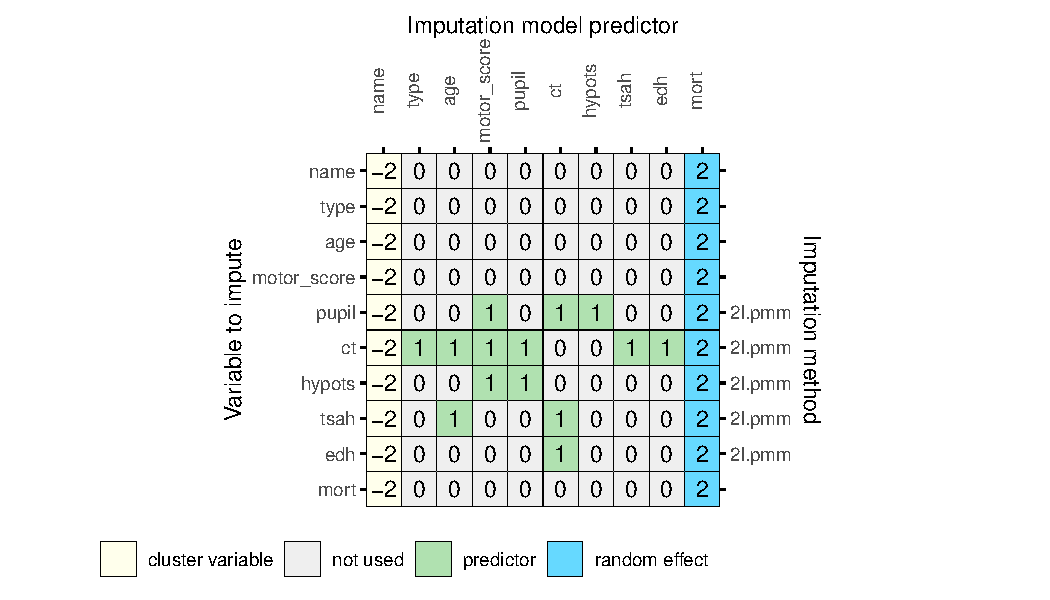
\includegraphics{manuscript_files/figure-pdf/unnamed-chunk-38-1.pdf}

}

\end{figure}

Impute the incomplete data with

\begin{verbatim}
R> imp <- mice(
+  dat,
+  method = meth,
+  predictorMatrix = pred,
+  printFlag = FALSE
+)
\end{verbatim}

Evaluate the convergence of the algorithm

\begin{verbatim}
R> plot_trace(imp)
\end{verbatim}

\begin{figure}[h]

{\centering 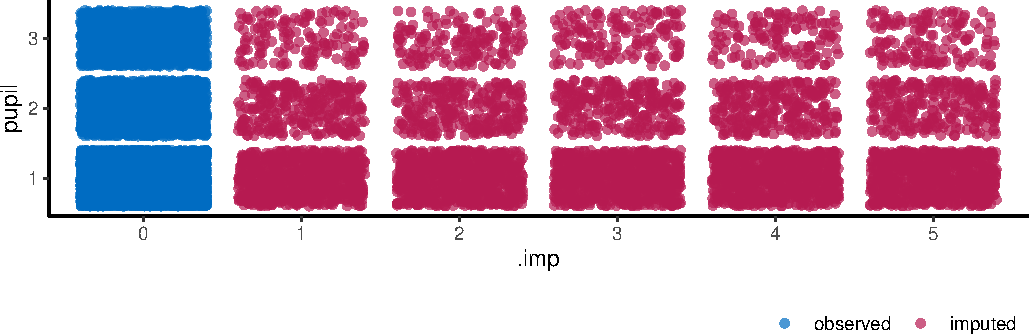
\includegraphics{manuscript_files/figure-pdf/unnamed-chunk-40-1.pdf}

}

\end{figure}

Evaluate the imputed values.

\begin{verbatim}
R> ggmice(imp, aes(.imp, pupil)) +
+  geom_jitter()
\end{verbatim}

\begin{figure}[h]

{\centering 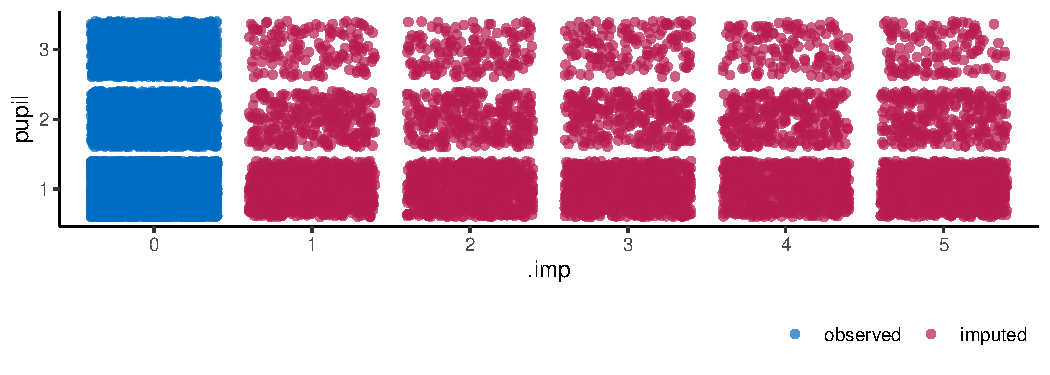
\includegraphics{manuscript_files/figure-pdf/unnamed-chunk-41-1.pdf}

}

\end{figure}

Convert the data back to factors.

\begin{verbatim}
long <- complete(imp, "long", include = TRUE)
long <- mutate(long, across(c("motor_score", "pupil", "ct"), as.factor))
imp <- as.mids(long)
\end{verbatim}

Analyze the imputed data:

\begin{verbatim}
R> fit <- imp %>%
+  with(glmer(
+    mort ~ type + age + motor_score + pupil + ct + (1 | name),
+    family = "binomial"
+    ))
\end{verbatim}

The estimated effects after imputation are presented in Table XYZ.

\begin{verbatim}
R> est <- testEstimates(as.mitml.result(fit), extra.pars = TRUE)
\end{verbatim}

Display results in table.

\begin{verbatim}
R> est$estimates |> 
+  round(3) |>
+  kable()
\end{verbatim}

\begin{longtable}[]{@{}
  >{\raggedright\arraybackslash}p{(\columnwidth - 14\tabcolsep) * \real{0.1605}}
  >{\raggedleft\arraybackslash}p{(\columnwidth - 14\tabcolsep) * \real{0.1111}}
  >{\raggedleft\arraybackslash}p{(\columnwidth - 14\tabcolsep) * \real{0.1235}}
  >{\raggedleft\arraybackslash}p{(\columnwidth - 14\tabcolsep) * \real{0.0988}}
  >{\raggedleft\arraybackslash}p{(\columnwidth - 14\tabcolsep) * \real{0.1358}}
  >{\raggedleft\arraybackslash}p{(\columnwidth - 14\tabcolsep) * \real{0.2222}}
  >{\raggedleft\arraybackslash}p{(\columnwidth - 14\tabcolsep) * \real{0.0741}}
  >{\raggedleft\arraybackslash}p{(\columnwidth - 14\tabcolsep) * \real{0.0741}}@{}}
\toprule\noalign{}
\begin{minipage}[b]{\linewidth}\raggedright
\end{minipage} & \begin{minipage}[b]{\linewidth}\raggedleft
Estimate
\end{minipage} & \begin{minipage}[b]{\linewidth}\raggedleft
Std.Error
\end{minipage} & \begin{minipage}[b]{\linewidth}\raggedleft
t.value
\end{minipage} & \begin{minipage}[b]{\linewidth}\raggedleft
df
\end{minipage} & \begin{minipage}[b]{\linewidth}\raggedleft
P(\textgreater\textbar t\textbar)
\end{minipage} & \begin{minipage}[b]{\linewidth}\raggedleft
RIV
\end{minipage} & \begin{minipage}[b]{\linewidth}\raggedleft
FMI
\end{minipage} \\
\midrule\noalign{}
\endhead
\bottomrule\noalign{}
\endlastfoot
(Intercept) & -1.892 & 0.333 & -5.682 & 11445.455 & 0.000 & 0.019 &
0.019 \\
type & -0.346 & 0.178 & -1.948 & 686356.768 & 0.051 & 0.002 & 0.002 \\
age & 0.032 & 0.002 & 19.564 & 2418.910 & 0.000 & 0.042 & 0.041 \\
motor\_score2 & -0.575 & 0.070 & -8.226 & 71295.018 & 0.000 & 0.008 &
0.008 \\
motor\_score3 & -0.891 & 0.072 & -12.440 & 66712.189 & 0.000 & 0.008 &
0.008 \\
motor\_score4 & -1.276 & 0.074 & -17.305 & 18426.087 & 0.000 & 0.015 &
0.015 \\
pupil2 & 1.315 & 0.068 & 19.339 & 110.826 & 0.000 & 0.235 & 0.204 \\
pupil3 & 0.657 & 0.075 & 8.745 & 423.463 & 0.000 & 0.108 & 0.101 \\
ct2 & 0.747 & 0.084 & 8.884 & 41.781 & 0.000 & 0.448 & 0.340 \\
ct3 & 0.766 & 0.090 & 8.535 & 12.103 & 0.000 & 1.352 & 0.631 \\
\end{longtable}

\begin{verbatim}
R> est$extra.pars |> 
+  round(3) |>
+  kable()
\end{verbatim}

\begin{longtable}[]{@{}lr@{}}
\toprule\noalign{}
& Estimate \\
\midrule\noalign{}
\endhead
\bottomrule\noalign{}
\endlastfoot
Intercept\textasciitilde\textasciitilde Intercept\textbar name &
0.082 \\
\end{longtable}

\hypertarget{obesity-data}{%
\subsection{obesity data}\label{obesity-data}}

In this example, we demonstrate a multilevel imputation of random
intercept and random slope model with a continuous response. We utilize
the obesity dataset included in the \texttt{micemd}@ package, a
simulated dataset that emulates an electronic survey in which
individuals are asked to provide information about their weight and
consumption habits in different countries. We simulate data for 5
clusters so that the true values are known. We use the following
variables from the dataset:

\begin{itemize}
\tightlist
\item
  \textbf{Cluster:} Region of the patients' healthcare provider (Cluster
  variable),
\item
  \textbf{Gender:} Subjects' Gender (0=male, 1=female),
\item
  \textbf{Age:} Subjects' age,
\item
  \textbf{Height:} Subjects' height in metres,
\item
  \textbf{Weight:} Subjects' weight in kilograms,
\item
  \textbf{BMI:} Subjects' body mass index,
\item
  \textbf{FamOb:} Family obesity history (yes or no),
\item
  \textbf{Time:} Response time in minutes (exclusion-restriction
  variable).
\end{itemize}

In this dataset, Age and FamOb are MAR, while the weight variable is
affected by selection bias, attributed to an indirect MNAR mechanism.
This MNAR mechanism typically arises when an unobserved or omitted
variable influences both the value of the incomplete variable (in this
case, Weight) and its likelihood of being missing (denoted as R).

In the primary analysis model, BMI serves as the dependent variable,
with Age, Gender, and FamOb as predictors. Because of the clustered
nature of the data, which is quantified with the Intraclass Correlation
Coefficient (ICC) below, we include random intercepts, as well as a
random slope for the Age variable. The model is represented as:
\begin{equation}
\label{eqn:main}
BMI_{ij}= (\beta_{o}+ b_{oj} ) + (\beta_{1}+ b_{oj})* Age_{ij} + \beta_{2}*FamOb_{ij}+ \beta_{3}Gender_{ij} + \epsilon_{ij}
\end{equation}

We start by loading the data:

\begin{verbatim}
R> data(Obesity, package = "micemd")
\end{verbatim}

Now, let's begin by examining the missing patterns in the data by
cluster:

\begin{verbatim}
R> plot_pattern(Obesity)
\end{verbatim}

\begin{figure}[h]

{\centering 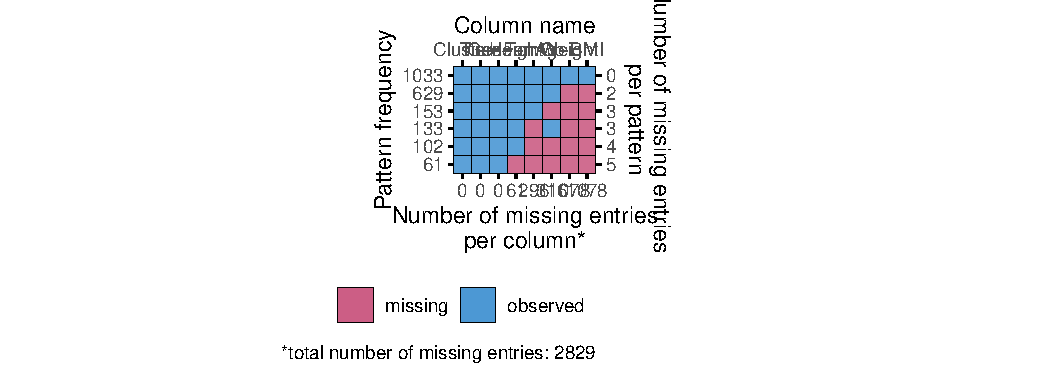
\includegraphics{manuscript_files/figure-pdf/unnamed-chunk-48-1.pdf}

}

\end{figure}

\begin{verbatim}
R> # Obesity |> 
R> #   split(~Cluster) |>
R> #   lapply(plot_pattern)
\end{verbatim}

We observe that the missing pattern is non-monotonic and quite similar
across the clusters. However, regarding the weight variable, we notice
that is systematically missing in cluster 3. In order to evaluate if we
require a imputation method that accounts for clustering we assess the
Intraclass Correlation

\begin{verbatim}
R> Nulmodel <- lmer(BMI ~ 1 + (1|Cluster), data = Obesity)
R> # performance::icc(Nulmodel)
\end{verbatim}

Since the ICC is above 0.1 and as the main analysis will be use a mixed
model, we decide to use two-level (2l) imputation methods. In this
imputation process, we include all predictor variables from equation
\ref{eqn:main} in the main model. However, since BMI is a composite of
weight and height, we use deterministic imputation for these, which is
described below.

We use the \textbf{find.defaultMethodfunction} provided in the
\textbf{micemd} package, which suggests an appropriate method for MAR
variables based on the type of variable, number of observations in the
cluster, and number of clusters.

It suggests using `2l.2stage.bin' for the FAV variable and
`2l.2stage.norm' for the age variable. However, after inspecting the age
density plot, we consider modifying its method to `2l.2stage.pmm'. For
the BMI variable, we employ deterministic imputation.

\begin{verbatim}
meth_mar <-
  find.defaultMethod(
    Obesity,
    ind.clust = 1,
    I.small = 7,
    ni.small = 100,
    prop.small = 0.4
  )
meth_mar["BMI"] <- "~ I(Weight / (Height)^2)"
meth_mar["Age"] <- "2l.2stage.pmm"
\end{verbatim}

For these imputation models, it is necessary to specify the prediction
matrix, with the cluster variable labelled as -2 and the predictor
variable measured within clusters labelled as 2, encompassing all
variables. We need to suprime the variable Time as this variable is not
specified in the main model. We also modify the relationship between
BMI, weight and height in the prediction matrix to avoid circular
predictions. Then we proceed to run the imputation model.

\begin{verbatim}
pred_mar <- quickpred(Obesity)
pred_mar[, "Cluster"] <- -2 
pred_mar[, "Time"] <- 0
pred_mar[pred_mar == 1] <- 2
pred_mar[c("Height", "Weight"), "BMI"] <- 0
plot_pred(pred_mar)
\end{verbatim}

\begin{figure}[h]

{\centering 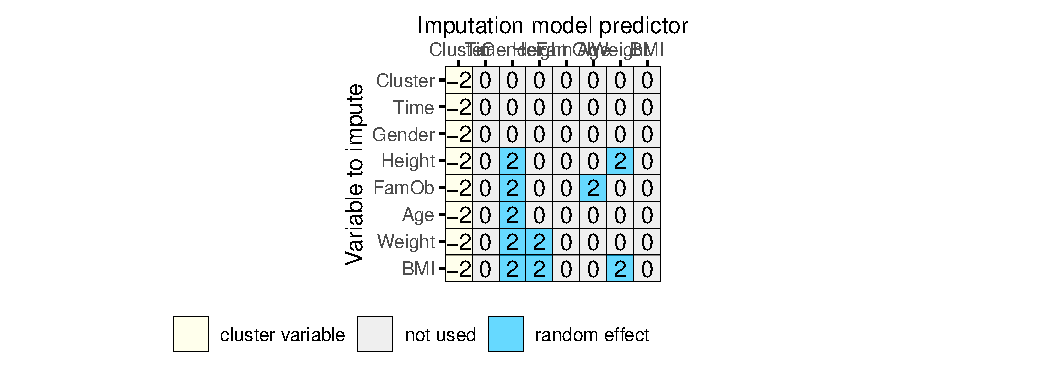
\includegraphics[width=0.7\textwidth,height=\textheight]{manuscript_files/figure-pdf/obesity-predmar-1.pdf}

}

\end{figure}

\begin{verbatim}
imp_mar <-
  mice(
    data = Obesity,
    method = meth_mar,
    predictorMatrix = pred_mar,
    printFlag = FALSE
  )
\end{verbatim}

\begin{verbatim}
summary(complete(imp_mar,"long")$Weight)
\end{verbatim}

\begin{verbatim}
   Min. 1st Qu.  Median    Mean 3rd Qu.    Max. 
  4.428  69.890  82.800  82.835  95.491 145.885 
\end{verbatim}

We are also contemplating the utilisation of the predictive mean
matching (pmm) option, as the values imputed using a fully parametric
method may be implausibly low for some patients.

\begin{verbatim}
meth_mar["Weight"] <- "2l.2stage.pmm"
imp_mar_pmm <- mice(
  data = Obesity,
  method = meth_mar,
  predictorMatrix = pred_mar,
  printFlag = FALSE
)
\end{verbatim}

\begin{verbatim}
summary(complete(imp_mar_pmm, "long")$Weight)
\end{verbatim}

\begin{verbatim}
   Min. 1st Qu.  Median    Mean 3rd Qu.    Max. 
  28.35   71.04   83.65   83.87   95.66  134.61 
\end{verbatim}

\begin{verbatim}
plot_trace(imp_mar_pmm, "Weight")
\end{verbatim}

\begin{figure}[h]

{\centering 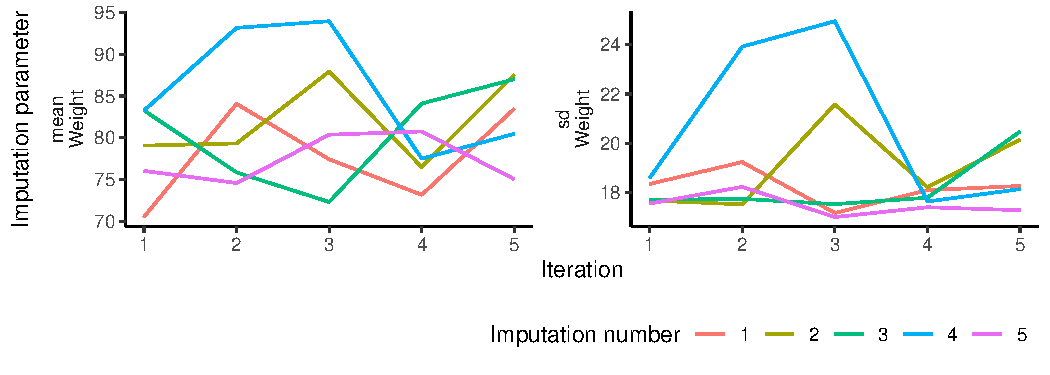
\includegraphics{manuscript_files/figure-pdf/obesity-predmar_pmm1-1.pdf}

}

\end{figure}

\begin{verbatim}
ggmice(imp_mar_pmm, aes(.imp, Weight)) + 
  geom_jitter()
\end{verbatim}

\begin{figure}[h]

{\centering 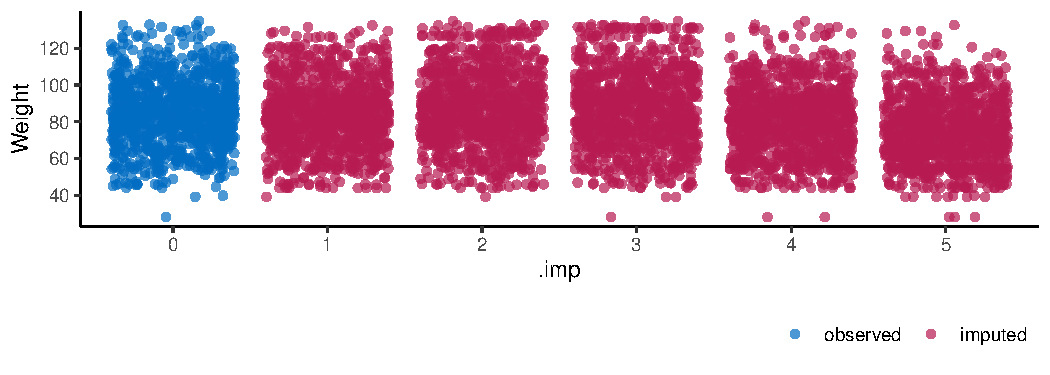
\includegraphics{manuscript_files/figure-pdf/obesity-predmar_pmm1-2.pdf}

}

\end{figure}

Analyze the imputed data.

\begin{verbatim}
R> # fit <- with(
R> #     imp_mar_pmm,
R> #     lme(BMI ~ Age + FamOb + Gender, random =  ~ 1 + Age | Cluster)
R> #     )
R> fit <- with(
+    imp_mar_pmm,
+    lmer(BMI ~ Age + FamOb + Gender + (1 + Age | Cluster))
+    )
R> est <- testEstimates(as.mitml.result(fit), extra.pars = TRUE)
\end{verbatim}

Display results in table.

\begin{verbatim}
R> est$estimates |> 
+  round(3) |>
+  kable()
\end{verbatim}

\begin{longtable}[]{@{}
  >{\raggedright\arraybackslash}p{(\columnwidth - 14\tabcolsep) * \real{0.1558}}
  >{\raggedleft\arraybackslash}p{(\columnwidth - 14\tabcolsep) * \real{0.1169}}
  >{\raggedleft\arraybackslash}p{(\columnwidth - 14\tabcolsep) * \real{0.1299}}
  >{\raggedleft\arraybackslash}p{(\columnwidth - 14\tabcolsep) * \real{0.1039}}
  >{\raggedleft\arraybackslash}p{(\columnwidth - 14\tabcolsep) * \real{0.1039}}
  >{\raggedleft\arraybackslash}p{(\columnwidth - 14\tabcolsep) * \real{0.2338}}
  >{\raggedleft\arraybackslash}p{(\columnwidth - 14\tabcolsep) * \real{0.0779}}
  >{\raggedleft\arraybackslash}p{(\columnwidth - 14\tabcolsep) * \real{0.0779}}@{}}
\toprule\noalign{}
\begin{minipage}[b]{\linewidth}\raggedright
\end{minipage} & \begin{minipage}[b]{\linewidth}\raggedleft
Estimate
\end{minipage} & \begin{minipage}[b]{\linewidth}\raggedleft
Std.Error
\end{minipage} & \begin{minipage}[b]{\linewidth}\raggedleft
t.value
\end{minipage} & \begin{minipage}[b]{\linewidth}\raggedleft
df
\end{minipage} & \begin{minipage}[b]{\linewidth}\raggedleft
P(\textgreater\textbar t\textbar)
\end{minipage} & \begin{minipage}[b]{\linewidth}\raggedleft
RIV
\end{minipage} & \begin{minipage}[b]{\linewidth}\raggedleft
FMI
\end{minipage} \\
\midrule\noalign{}
\endhead
\bottomrule\noalign{}
\endlastfoot
(Intercept) & 28.445 & 2.262 & 12.578 & 158.191 & 0.000 & 0.189 &
0.169 \\
Age & 0.041 & 0.032 & 1.312 & 383.212 & 0.190 & 0.114 & 0.107 \\
FamObyes & 0.000 & 0.316 & -0.001 & 207.642 & 0.999 & 0.161 & 0.147 \\
GenderMale & -1.361 & 0.411 & -3.310 & 7.985 & 0.011 & 2.422 & 0.761 \\
\end{longtable}

\begin{verbatim}
R> est$extra.pars |> 
+  round(3) |>
+  kable()
\end{verbatim}

\begin{longtable}[]{@{}lr@{}}
\toprule\noalign{}
& Estimate \\
\midrule\noalign{}
\endhead
\bottomrule\noalign{}
\endlastfoot
Intercept\textasciitilde\textasciitilde Intercept\textbar Cluster &
19.862 \\
Age\textasciitilde\textasciitilde Age\textbar Cluster & 0.002 \\
Intercept\textasciitilde\textasciitilde Age\textbar Cluster & -0.067 \\
Residual\textasciitilde\textasciitilde Residual & 26.010 \\
ICC\textbar Cluster & 0.395 \\
\end{longtable}

After confirming convergence, we proceed to save the results for future
use. We consider the possibility that patients may not have been
selected randomly, which would then have led to a distribution for
weight that does not reflect the weight in the population. It???s likely
that an omitted variable, like self-esteem, could influence this
selection. For instance, individuals with lower self-esteem might have
higher weight values, impacting their willingness to provide honest
information due to embarrassment.

To address this situation, two approaches have been proposed for dealing
with Missing Not at Random (MNAR) data: pattern-mixed models and
selection models. Within pattern-mixed models, methods like the delta
method and more advanced ones like NARFS have been suggested. The
selection model approach includes methods such as the Heckman model,
which can be particularly useful in this case. Several methods,
including those by \cite{galimard2018}, and the recently a Heckman
method designed for two-level data, allow for variations in intercepts
and exposure effects (random intercept and slope) \cite{munoz2023}.

To apply the \textbf{2l.2stage.heckman} method, the weight variable
should be specified as `2l.2stage.heckman' found in the micemd package.
Additionally, the prediction matrix needs modification because this
method involves specifying two equations: one for the outcome,
describing the incomplete variable in terms of partially observed
predictors (in this case, all variables from the main model), and the
other for the selection model, explaining the probability of being
observed based (R) on certain variables. For the outcome equation we
consider the same imputation model that we used for the MAR case (main
model).
\[Weight_{ij}= \beta^O_{o} + \beta^O_{1}Age_{ij} + \beta^O_{2}FamOb_{ij}+ \beta^O_{3}Gender_{ij} + \epsilon^O_{ij}\]
Regarding the selection equation, we include the same predictors as
those in the main model, as well as a time variable. Here the time
variable serves as a restriction exclusion variable specifically
explaining the probability of being observed but not affecting the
incomplete value (Weight). In this context, we assume that the time a
user spends completing the survey serves as a proxy for the barriers
they may encounter in survey completion, such as familiarity with the
survey content or internet speed. These factors may lead the user to
skip specific questions or even the entire survey. Also, we assume the
time does not have any influence on the subject???s weight.
\[R_{ij}= \beta^S_{o} + \beta^S_{1}Age_{ij} + \beta^S_{2}FamOb_{ij}+ \beta^S_{3}Gender_{ij} +\beta^S_{4}Time_{ij}+ \epsilon^S_{ij}\]

These two equations are jointly estimated under the assumption that the
error terms are interconnected with a bivariate normal distribution. For
a more comprehensive understanding of the model and the exclusion
restriction, see \cite{munoz2023a}.

To use information from both equations, we must adjust the prediction
matrix. The cluster variable remains specified as before (-2). In this
imputation method, all the variables present in both the selection and
outcome equations are included with a random effect.

However, it is essential to distinguish which of these variables appear
in each equation. In this framework, when a variable is shared between
both equations, it is denoted as (2). Predictors exclusive to the
outcome equation are indicated as (-4), while those exclusive to the
selection equation are labelled as (-3). Consequently, the only
alteration needed in the predictor matrix pertains to the variable
`Time'.

\begin{verbatim}
pred_mnar <- pred_mar
pred_mnar["Weight","Time"] <- -3
plot_pred(pred_mnar)
\end{verbatim}

\begin{figure}[h]

{\centering 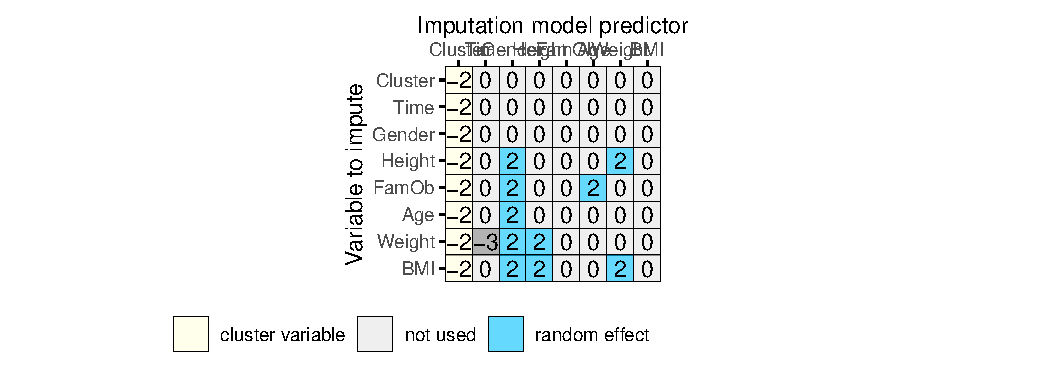
\includegraphics{manuscript_files/figure-pdf/obesity-predmnar-1.pdf}

}

\end{figure}

We also need to modify the method of the weight variable.

\begin{verbatim}
meth_mnar <- meth_mar
meth_mnar["Weight"] <- "2l.2stage.heckman"
\end{verbatim}

Then we proceed to run the imputation model as before, after executing
these imputation procedures, it is essential to assess convergence and
the coherence of the imputed values.

\begin{verbatim}
imp_mnar <- mice(
  data = Obesity,
  method = meth_mnar,
  predictorMatrix = pred_mnar,
  printFlag = FALSE
)
summary(complete(imp_mnar, "long")$Weight)
\end{verbatim}

\begin{verbatim}
   Min. 1st Qu.  Median    Mean 3rd Qu.    Max. 
  16.26   70.95   85.21   86.14  100.14  190.95 
\end{verbatim}

Upon examining the weight variable, we noticed that the imputed range
falls outside the realm of plausible values (as weight should be
positive).

\begin{verbatim}
summary(complete(imp_mnar, "long")$Weight)
\end{verbatim}

\begin{verbatim}
   Min. 1st Qu.  Median    Mean 3rd Qu.    Max. 
  16.26   70.95   85.21   86.14  100.14  190.95 
\end{verbatim}

Consequently, as before we use the `pmm', option but this time for the
Heckman imputation, this approach ensures that the imputed values remain
within the range of observable values. We then run the imputation model
but this time using the option of pmm, to assure that weight values are
in the range of the observable data, this can be implemented by setting
the pmm parameter to true.

\begin{verbatim}
imp_mnar_pmm <-
  mice(
    data = Obesity,
    method = meth_mnar,
    predictorMatrix = pred_mnar,
    pmm = T,
    printFlag = FALSE
  )
\end{verbatim}

We check the convergence of the results

\begin{verbatim}
summary(complete(imp_mnar_pmm, "long")$Weight)
\end{verbatim}

\begin{verbatim}
   Min. 1st Qu.  Median    Mean 3rd Qu.    Max. 
  28.35   71.51   85.07   85.35   98.90  134.61 
\end{verbatim}

\begin{verbatim}
plot_trace(imp_mar_pmm, "Weight")
\end{verbatim}

\begin{figure}[h]

{\centering 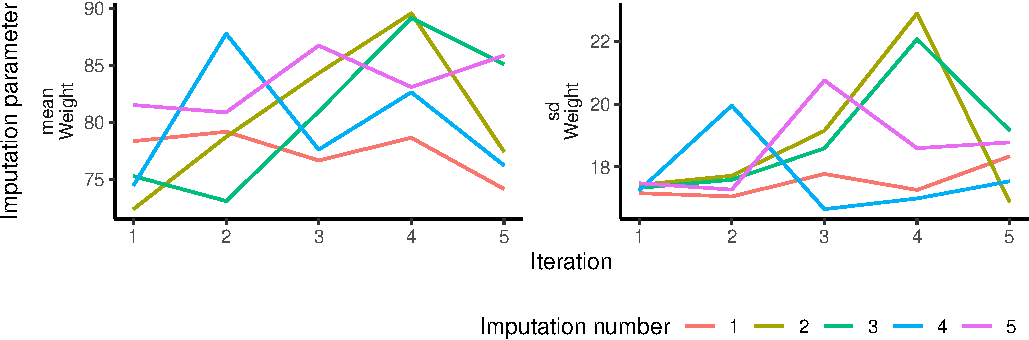
\includegraphics{manuscript_files/figure-pdf/obesity-predmnarp1-1.pdf}

}

\end{figure}

After this modification we proceed to compare the effects on the model.
We run the analysis model on each of the completed datasets as well as
the dataset where the incomplete values are removed (Complete Case
analysis, CC).

\begin{verbatim}
# cc_rs <- with(setDT(Obesity)[complete.cases(Obesity), ],
#               lme(BMI ~ Age + FamOb + Gender, random =  ~ 1 + Age |
#                     Cluster))
mar_rs <- with(
  imp_mar, 
  lme(BMI ~ Age + FamOb + Gender, random =  ~ 1 + Age | Cluster)
  )
mar_pmm_rs <- with(
    imp_mar_pmm,
    lme(BMI ~ Age + FamOb + Gender, random =  ~ 1 + Age | Cluster)
    )
mnar_rs <- with(
  imp_mnar, 
  lme(BMI ~ Age + FamOb + Gender, random =  ~ 1 + Age | Cluster)
  )
mnar_pmm_rs <- with(
  imp_mnar_pmm,
  lme(BMI ~ Age + FamOb + Gender, random =  ~ 1 + Age | Cluster)
  )
# list_models <- list(cc_rs, mar_rs, mar_pmm_rs, mnar_rs, mnar_pmm_rs)
# plot_models(list_models,
#             mod_name = c("Complete case", "MAR", "MAR_pmm", "MNAR", "MNAR_pmm"))
\end{verbatim}

\begin{verbatim}
est <- testEstimates(as.mitml.result(mnar_pmm_rs), extra.pars = TRUE)
\end{verbatim}

Display results in table.

\begin{verbatim}
R> est$estimates |> 
+  round(3) |>
+  kable()
\end{verbatim}

\begin{longtable}[]{@{}
  >{\raggedright\arraybackslash}p{(\columnwidth - 14\tabcolsep) * \real{0.1558}}
  >{\raggedleft\arraybackslash}p{(\columnwidth - 14\tabcolsep) * \real{0.1169}}
  >{\raggedleft\arraybackslash}p{(\columnwidth - 14\tabcolsep) * \real{0.1299}}
  >{\raggedleft\arraybackslash}p{(\columnwidth - 14\tabcolsep) * \real{0.1039}}
  >{\raggedleft\arraybackslash}p{(\columnwidth - 14\tabcolsep) * \real{0.0909}}
  >{\raggedleft\arraybackslash}p{(\columnwidth - 14\tabcolsep) * \real{0.2338}}
  >{\raggedleft\arraybackslash}p{(\columnwidth - 14\tabcolsep) * \real{0.0909}}
  >{\raggedleft\arraybackslash}p{(\columnwidth - 14\tabcolsep) * \real{0.0779}}@{}}
\toprule\noalign{}
\begin{minipage}[b]{\linewidth}\raggedright
\end{minipage} & \begin{minipage}[b]{\linewidth}\raggedleft
Estimate
\end{minipage} & \begin{minipage}[b]{\linewidth}\raggedleft
Std.Error
\end{minipage} & \begin{minipage}[b]{\linewidth}\raggedleft
t.value
\end{minipage} & \begin{minipage}[b]{\linewidth}\raggedleft
df
\end{minipage} & \begin{minipage}[b]{\linewidth}\raggedleft
P(\textgreater\textbar t\textbar)
\end{minipage} & \begin{minipage}[b]{\linewidth}\raggedleft
RIV
\end{minipage} & \begin{minipage}[b]{\linewidth}\raggedleft
FMI
\end{minipage} \\
\midrule\noalign{}
\endhead
\bottomrule\noalign{}
\endlastfoot
(Intercept) & 28.880 & 2.391 & 12.078 & 56.876 & 0.000 & 0.361 &
0.290 \\
Age & 0.050 & 0.037 & 1.343 & 19.874 & 0.194 & 0.814 & 0.497 \\
FamObyes & -0.027 & 0.490 & -0.056 & 11.685 & 0.957 & 1.410 & 0.642 \\
GenderMale & -1.484 & 0.804 & -1.846 & 4.813 & 0.126 & 10.318 & 0.934 \\
\end{longtable}

\begin{verbatim}
R> est$extra.pars |> 
+  round(3) |>
+  kable()
\end{verbatim}

\begin{longtable}[]{@{}lr@{}}
\toprule\noalign{}
& Estimate \\
\midrule\noalign{}
\endhead
\bottomrule\noalign{}
\endlastfoot
Intercept\textasciitilde\textasciitilde Intercept\textbar Cluster &
19.111 \\
Age\textasciitilde\textasciitilde Age\textbar Cluster & 0.001 \\
Intercept\textasciitilde\textasciitilde Age\textbar Cluster & -0.046 \\
Residual\textasciitilde\textasciitilde Residual & 30.071 \\
ICC\textbar Cluster & 0.372 \\
\end{longtable}

We note that there is minimal disparity in the age effect, FamObs, or
Gender across the various imputation models under consideration. An
analysis of the intercept reveals that, under the MNAR assumption, a
higher average BMI is anticipated compared to the MAR assumption.
Nonetheless, with respect to precision of estimates, we notice that in
general MNAR imputation leads to wider confidence intervals, in this
case it does not have any influence on the final result but there could
be cases where variation in the assumed missing mechanism could lead
also to differences on significant test and therefore lead to
contradictory conclusions.

\hypertarget{conclusion}{%
\section{Conclusion}\label{conclusion}}

This paper is dedicated to exploring the imputation process for
incomplete datasets, with a primary focus on utilizing a hierarchical
model for analysis. Initially, users are encouraged to consider the main
analysis within the context of the incomplete dataset, along with
insights provided by domain experts, to gain a better understanding of
variable relationships. Employing clear data visualization is
instrumental in comprehending the missing data patterns, establishing a
missing mechanism, and aiding in the selection of suitable imputation
methods.

The ``Mice'' and ``mice''-based R packages offer a range of imputation
methods tailored for hierarchical data, easily adaptable to the
dataset's structure. Before proceeding with the analysis of the imputed
dataset, it is essential to assess the convergence of the imputation
method. This evaluation can reveal issues such as circular problems, the
need for additional iterations, or challenges associated with the chosen
imputation method.

\hypertarget{funding}{%
\section{Funding}\label{funding}}

This project has received funding from the European Union's Horizon 2020
research and innovation programme under ReCoDID grant agreement No
825746.

The views expressed in this paper are the personal views of the authors
and may not be understood or quoted as being made on behalf of or
reflecting the position of the regulatory agency/agencies or
organizations with which the authors are employed/affiliated.

\hypertarget{sec-summary}{%
\section{Summary and discussion}\label{sec-summary}}

What is missing from this manuscript\ldots{}

\hypertarget{computational-details}{%
\section*{Computational details}\label{computational-details}}
\addcontentsline{toc}{section}{Computational details}

The results in this paper were obtained using
\proglang{R}\textasciitilde4.3.0. \proglang{R} itself and all packages
used are available from the Comprehensive \proglang{R} Archive Network
(CRAN) at {[}https://CRAN.R-project.org/{]}.

\hypertarget{acknowledgments}{%
\section*{Acknowledgments}\label{acknowledgments}}
\addcontentsline{toc}{section}{Acknowledgments}

This project has received funding from the European Union's Horizon 2020
research and innovation programme under ReCoDID grant agreement No
825746.

\hypertarget{references}{%
\section*{References}\label{references}}
\addcontentsline{toc}{section}{References}

\renewcommand{\bibsection}{}
\bibliography{bibliography.bib}

\newpage{}

\hypertarget{sec-techdetails}{%
\section*{More technical details}\label{sec-techdetails}}
\addcontentsline{toc}{section}{More technical details}

\begin{tcolorbox}[enhanced jigsaw, toprule=.15mm, arc=.35mm, rightrule=.15mm, breakable, opacityback=0, bottomrule=.15mm, colback=white, leftrule=.75mm, left=2mm]

Appendices can be included after the bibliography (with a page break).
Each section within the appendix should have a proper section title
(rather than just \emph{Appendix}).

For more technical style details, please check out JSS's style FAQ at
{[}https://www.jstatsoft.org/pages/view/style\#frequently-asked-questions{]}
which includes the following topics:

\begin{itemize}
\tightlist
\item
  Title vs.~sentence case.
\item
  Graphics formatting.
\item
  Naming conventions.
\item
  Turning JSS manuscripts into \proglang{R} package vignettes.
\item
  Trouble shooting.
\item
  Many other potentially helpful details\ldots{}
\end{itemize}

\end{tcolorbox}

\hypertarget{sec-bibtex}{%
\section*{Using BibTeX}\label{sec-bibtex}}
\addcontentsline{toc}{section}{Using BibTeX}

\begin{tcolorbox}[enhanced jigsaw, toprule=.15mm, arc=.35mm, rightrule=.15mm, breakable, opacityback=0, bottomrule=.15mm, colback=white, leftrule=.75mm, left=2mm]

References need to be provided in a \textsc{Bib}{\TeX} file
(\texttt{.bib}). All references should be made with \texttt{@cite}
syntax. This commands yield different formats of author-year citations
and allow to include additional details (e.g.,pages, chapters, \dots) in
brackets. In case you are not familiar with these commands see the JSS
style FAQ for details.

Cleaning up \textsc{Bib}{\TeX} files is a somewhat tedious task --
especially when acquiring the entries automatically from mixed online
sources. However, it is important that informations are complete and
presented in a consistent style to avoid confusions. JSS requires the
following format.

\begin{itemize}
\tightlist
\item
  item JSS-specific markup (\texttt{\textbackslash{}proglang},
  \texttt{\textbackslash{}pkg}, \texttt{\textbackslash{}code}) should be
  used in the references.
\item
  item Titles should be in title case.
\item
  item Journal titles should not be abbreviated and in title case.
\item
  item DOIs should be included where available.
\item
  item Software should be properly cited as well. For \proglang{R}
  packages \texttt{citation("pkgname")} typically provides a good
  starting point.
\end{itemize}

\end{tcolorbox}




\end{document}
